%%%%%%%%%%%%%%%%%%%%%%%%%%%%% TCC %%%%%%%%%%%%%%%%%%%%%%%%%%%%%%%%
%
% Template para TCC da Universidade Federal da Paraíba
%
% Autores: Elaine Soares elaineanita1@gmail.com
%          Rafael Brayner rafabrayner92@gmail.com
%          Roberto Júnior contato@robertojunior.net
% 
% Revisão: Eudisley Anjos eudisley@ci.ufpb.br
%
% Sinta-se livre para melhorar e contribuir com esse projeto. 
%
%%%%%%%%%%%%%%%%%%%%%%%%%%%%%%%%%%%%%%%%%%%%%%%%%%%%%%%%%%%%%%%%%%%

\documentclass{tcc}

\begin{document}
\pagestyle{empty} %retira numeração da página
%Dados do TCC%
\author{João Wallace Lucena Lins}
\title{colcom: Uma plataforma web participativa para a deliberação coletiva e desenvolvimento de ideias}
\newcommand{\subtitulo}{Subtítulo}
\newcommand{\nomedocurso}{Engenharia da Computação}
\newcommand{\titulobar}{titulo}
\newcommand{\orientador}{Yuri de Almeida Malheiros Barbosa}
\newcommand{\profa}{Yuri de Almeida Malheiros Barbosa}
\newcommand{\profb}{Thaís Gaudencio do Rêgo}
\newcommand{\profc}{Alexandre Nóbrega Duarte}
\newcommand{\insta}{Universidade Federal da Paraíba}
\newcommand{\instb}{Universidade Federal da Paraíba}
\newcommand{\instc}{Universidade Federal da Paraíba}
\newcommand{\coordenador}{Nome do Coordenador}
\newcommand{\departamento}{Nome do Departamento}

\begin{center}
\LARGE{\bf \thetitle}\\
% \Large{\bf \subtitulo}\\
\end{center}

\vspace{1em}

\begin{center}
\theauthor
\end{center}

\vfill


\begin{figure}[H]
\centering
% 
\includegraphics{imagens/logo2.jpg}

\includegraphics[width=0.18\linewidth]{imagens/logo_ci.png}
\end{figure}

\begin{center}
CENTRO DE INFORMÁTICA \\
UNIVERSIDADE FEDERAL DA PARAÍBA

\end{center}

\vspace{2in}

\begin{center}
João Pessoa, PB

\the\year
\end{center}
\afterpage{ \addtocounter{page}{1}} %addtocounter incrementa numero da pagina ja que blankpage nao entra no contador%

\newpage
\begin{center}
\theauthor
\end{center}
\vspace{3in}
\begin{center}
\LARGE{\thetitle}\\
\end{center}

\vspace{2in}

\begin{flushright}
Relatório Técnico apresentado ao curso \nomedocurso \\ do Centro de Informática, da Universidade Federal da Paraíba, \\ como requisito para a obtenção do grau de Bacharel em \nomedocurso
\\
\vspace{0.2in}

Orientador: \orientador


\end{flushright}

\vfill
\begin{center}
\MONTH de \the\year
\end{center}

% \newpage

% $ $
% \vfill


% \begin{flushright}
% \fbox{\parbox[t][15em][c]{0.90\linewidth}{
% \vspace{0.5in}

% $\qquad$ Ficha catalográfica: elaborada pela biblioteca do CI. 
% \vspace{0.15in}

% $\qquad$ Será impressa no verso da folha de rosto e não deverá ser contada. 

% $\qquad$ Se não houver biblioteca, deixar em branco.
% }}
% \end{flushright}

% \newpage

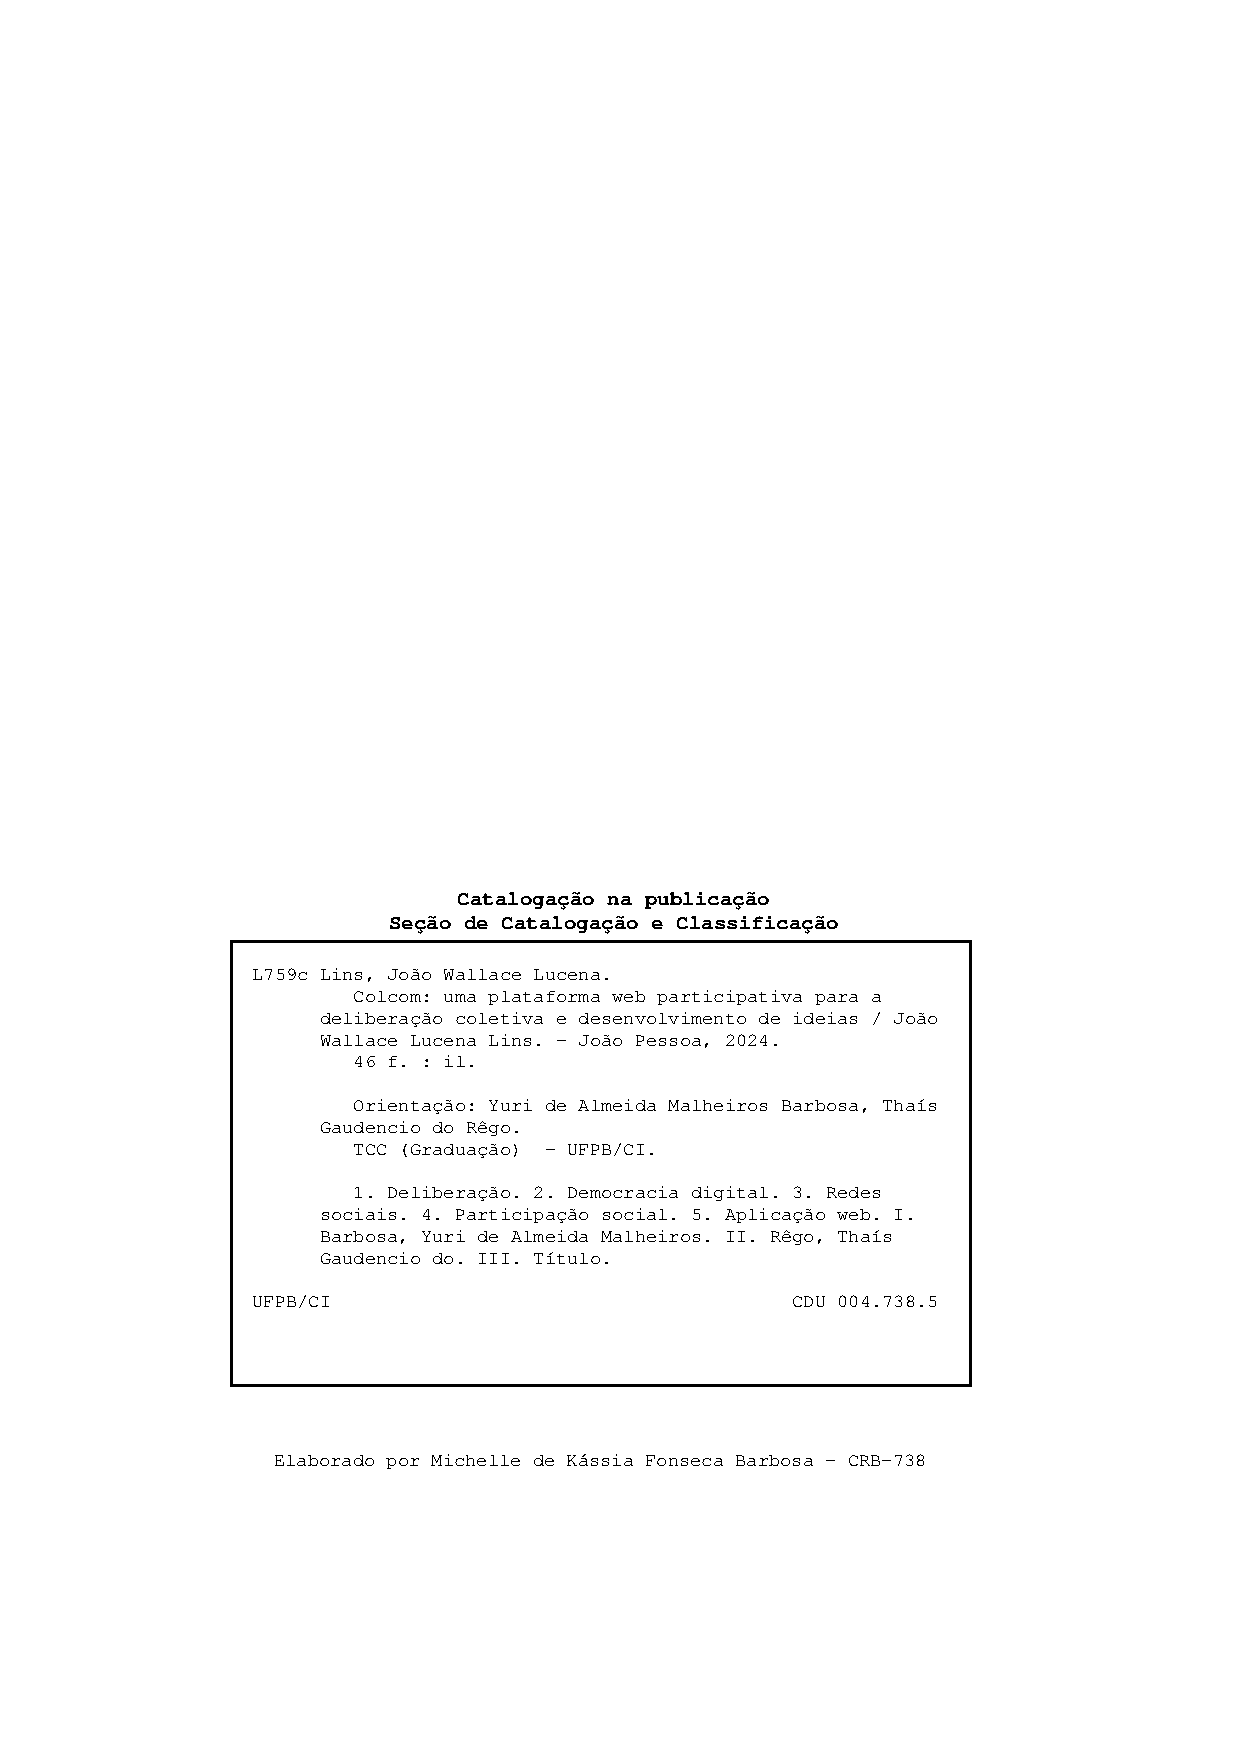
\includepdf{imagens/ficha_catalografica_54563.pdf}

\begin{figure}[H]
\centering
% 
\includegraphics{imagens/logo3.jpg}

\includegraphics[width=0.12\linewidth]{imagens/logo_ci.png}
\end{figure}

\begin{center}
CENTRO DE INFORMÁTICA \\
UNIVERSIDADE FEDERAL DA PARAÍBA
\end{center}

\vspace{0.05in}

Trabalho de Conclusão de Curso de {\nomedocurso} intitulado \textit{\bf \em \thetitle} de autoria de \theauthor, aprovada pela banca examinadora constituída pelos seguintes professores: \\

\vspace{0.7in}

\hrule
\noindent Prof. Dr. \profa\\
\insta\\

\vspace{0.25in}

\hrule
\noindent Prof. Dra. \profb\\
\instb\\

\vspace{0.25in}

\hrule
\noindent Prof. Dr. \profc\\
\instc\\

\vspace{0.8in}


\vfill

\begin{center}
João Pessoa, \today
\end{center}

\vspace{0.05in}

\begin{center}
\footnotesize{ Centro de Informática, Universidade Federal da Paraíba\\
Rua dos Escoteiros, Mangabeira VII, João Pessoa, Paraíba, Brasil CEP: 58058-600\\
Fone: +55 (83) 3216 7093 / Fax: +55 (83) 3216 7117}
\end{center}
\afterpage{ \addtocounter{page}{1}}
%página em branco%
\newpage
$ $
\vfill

\begin{flushright}
\em A minha família, amigos e povo do Brasil.
\end{flushright}

% \begin{flushright}
% Ao BaianaSystem
% \end{flushright}


\afterpage{ \addtocounter{page}{1}}

\newpage

%Dedicatória%
% \section*{\centering{DEDICATÓRIA}} 
% ***A dedicatória é opcional***

% \newpage

%Agradecimentos%
\section*{\centering{AGRADECIMENTOS}} 
Primeiramente, gostaria de agradecer a meus pais, José Wallace e Ivônia, pois sem seu apoio e influência não seria quem sou hoje e não poderia sequer sonhar em conquistar o que conquistei.

Em seguida, agradeço meu irmão Chrístian por ser uma companhia sempre presente em minha vida, e por ser sempre o primeiro a testar os limites das minhas ideias.

Não posso deixar de agradecer aos meus outros familiares, tios, tias, primos, primas, avós e avôs falecidos, e inclusive aos meus amigos — os quais considero minha segunda família —, cada um deles que me marcou e me moldou de alguma forma.

Também agradeço a Hevelyn Mafra, por ter sido uma namorada amorosa e companheira, sendo um grande apoio para mim durante a produção deste trabalho e de boa parte de minha graduação.

Agradeço ao meu orientador Dr. Yuri Malheiros, pela disponibilidade e solicitude, o que me habilitou a fazer este trabalho com segurança. Ademais, também o agradeço por ter sido um supervisor prestativo durante os projetos em que trabalhamos juntos.

Agradeço a minha professora e examinadora Dra. Thaís Gaudêncio, que, além de me ajudar enormemente na formulação do presente trabalho e a lidar com as burocracias com o processo de conclusão de curso, foi a primeira a me cativar para a área e acompanhou boa parte de minha trajetória na graduação;

Agradeço ao Dr. Alexandre Duarte, que prontamente aceitou o convite para participar da banca.

Agradeço a meus outros professores e mentores durante o curso, Anand Subramanian, que me aconselhou extensamente durante minha graduação; Marcelo Iury e Telmo Filho, que me guiaram muitas vezes em minhas experiências profissionais.

Agradeço, também, aos meus amigos que conheci durante minha graduação, principalmente João Pedro e Itamar, os quais foram influências muito positivas para meu desenvolvimento no curso e tornaram o peso do estudo um pouco menor.

Por fim, agradeço a todos que não me auxiliaram diretamente, mas que sem sua contribuição meu trabalho não seria possível: todos os trabalhadores da UFPB, todos os desenvolvedores que divulgam seus códigos e promovem o cenário \textit{open-source} e todos aqueles que visaram ampliar o papel do povo nas decisões políticas.

\newpage

%Resumo%
\section*{\centering{RESUMO}}
% Um resumo de trabalho de conclusão de curso é do tipo informativo e deve conter somente um parágrafo. A estrutura do resumo deve conter essencialmente os seguintes tópicos: apresentar inicialmente os objetivos do trabalho (o que foi feito?), a justificativa (porquê foi feito) e, finalmente, os resultados alcançados. O resumo deve informar ao leitor todas as informações importantes para o que o leitor possa entender o trabalho desenvolvido, quais foram as finalidades, a metodologia que o autor utilizou e os resultados obtidos. Deve conter frases curtas, porém completas (evitar estilo telegráfico); usar o tempo verbal no passado para os principais resultados e presente para comentários ou para salientar implicações significativas.  O resumo em português e inglês são obrigatórios e não devem passar de 200 palavras.

% Redes sociais são plataformas online que visam conectar usuários, permitindo-os compartilhar conteúdos e interagir entre si.
% O presente relatório técnico descreve o processo de projeto, implementação e validação da aplicação de código aberto colcom, a qual tem como intuito principal ser um ambiente favorável para a participação e deliberação de indivíduos de uma certa comunidade em seus processos de decisão, promovendo assim a democracia digital. A plataforma utiliza de práticas de redes sociais e conceitos de Sistemas de Controle de Versão (SCV), particularmente o \textit{Git}, como principais diretrizes de funcionamento.

% \noindent xxxxxxxx O presente relatório técnico descreve o processo de projeto, implementação e validação da aplicação de código aberto colcom. Seu intuito principal é ser um ambiente favorável para a participação e deliberação de indivíduos de uma certa comunidade em seus processos de decisão, promovendo, assim, a democracia digital. A plataforma utiliza práticas de redes sociais e conceitos de Sistemas de Controle de Versão (SCV), particularmente o \textit{Git}, como principais diretrizes de funcionamento.


% \noindent XXXXX 
\noindent Ferramentas de participação digital já são uma realidade no Brasil e em outros países, contudo, seu acesso ainda se restringe a uma pequena parcela dos usuários de internet; redes sociais por outro lado já são bem difundidas, mas sofrem de limitações significativas no que tange à deliberação eficaz. O objetivo principal da plataforma aqui proposta é ser um ambiente favorável para a participação e deliberação de indivíduos de uma certa comunidade em seus processos de decisão, promovendo, assim, a democracia digital em escala local. O presente relatório técnico descreve o processo de projeto, implementação e validação da aplicação de código aberto \textit{colcom}. A plataforma utiliza dinâmicas de redes sociais e conceitos de Sistemas de Controle de Versão (SCV), particularmente o \textit{Git}, como principais diretrizes de funcionamento.

{\bf Palavras-chave:} deliberação, democracia digital,  redes sociais, participação social, aplicação web.


\newpage

%Abstract%
\section*{\centering{ABSTRACT}} 
\noindent Digital participation tools are already a reality in Brazil and other countries, however, their access is still restricted to a small portion of internet users; Social networks, on the other hand, are already widespread, but suffer from significant limitations in terms of effective deliberation. The main objective of the platform here proposed is to be a favorable environment for the participation and deliberation of individuals from a certain community in their decision-making processes, thus promoting digital democracy on a local scale. This technical report describes the design, implementation and validation process of the \textit{colcom} open source application. The platform uses social network dynamics and Version Control Systems (VCS) concepts, particularly \textit{Git}, as its main operating guidelines.

{\bf Key-words:} deliberation, digital democracy, social networks, social participation, web application.

\newpage

%Lista de figuras%
\renewcommand{\listfigurename}{\centering LISTA DE FIGURAS}
\listoffigures
\newpage

%Lista de tabelas%
\renewcommand{\listtablename}{\centering LISTA DE TABELAS}
\listoftables
\newpage

%Lista de abreviaturas%
\section*{\centering{LISTA DE ABREVIATURAS}} 

CSS		–	\textit{Cascading Style Sheets}

HTML		– 	\textit{Hypertext Markup Language}

HTTP	–  	\textit{Hypertext Transfer Protocol}

JS	–  	\textit{JavaScript}

JSON	–  	\textit{JavaScript Object Notation}

JSX	–  	\textit{JavaScript XML}

LGPD	–  	Lei Geral de Proteção de Dados Pessoais

% MVP	–  	\textit{Model-View-Presenter}

SCV	–  	Sistema de controle de versões

SGBD	–  	Sistema gerenciador de banco de dados

SQL	–  	\textit{Structured Query Language}

Sass	–  	\textit{Syntactically Awesome Style Sheets}

TS	–  	\textit{TypeScript}












\newpage

%Sumário%

\pagestyle{plain} %mostra numeração da página%
\tableofcontents

\newpage
\section{INTRODUÇÃO}

A democracia digital é um conceito que começou a ser formulado após o advento e expansão da internet — que ocorreu concomitantemente à popularização de dispositivos que fazem uso dela, como computadores pessoais e aparelhos celulares —  e que vem se modernizando e concretizando juntamente com o desenvolvimento tecnológico. Valendo-se desta difusão do acesso à internet, foram propostas, nacionalmente e internacionalmente, diversas ferramentas que visam expandir a prática da democracia.

No cenário internacional, um dos maiores exemplos é o sistema \textit{Pol.is}\footnote{Disponível em: https://pol.is/. Acesso em: 25 de março de 2024.} \cite{polis} que já foi utilizado em 9 países diferentes, sendo o seu caso de uso de maior destaque em Taiwan, com o processo \textit{vTaiwan}\footnote{Disponível em: https://info.vtaiwan.tw/. Acesso em: 25 de março de 2024.}, iniciado em 2014, em que, de acordo com seu próprio \textit{website}, já foram discutidas mais de 28 pautas por mais de 200 mil participantes. 80\% dessas discussões levaram à alguma ação governamental decisiva.

No cenário nacional, o projeto de maior destaque é a plataforma \textit{Brasil Participativo}\footnote{Disponível em: https://brasilparticipativo.presidencia.gov.br/. Acesso em: 25 de março de 2024.}, que tem o título de maior experiência de participação social na internet já realizada pelo governo federal \cite{brasilParticipativo}. O projeto contou com mais de 1,4 milhões de participantes em sua primeira iniciativa digital de participação, o Plano Plurianual Participativo 2024 - 2027, em que os ministérios tiveram a responsabilidade de analisar os conteúdos propostos. Em seguida, o Ministério do Planejamento e Orçamento elaborou um documento de devolutiva contendo o que foi incorporado e a justificativa do que não foi incorporado, e por fim, o plano foi instituído na lei 14.802/2024\footnote{Disponível em: http://planalto.gov.br/ccivil\_03/\_ato2023-2026/2024/lei/L14802.htm. Acesso em: 1 abril de 2024.}, sancionada pelo presidente Lula. 

Entretanto, ainda há uma grande defasagem na adoção destas ferramentas pela população em geral, angariando somente uma pequena parcela dos usuários da internet, que ainda sequer constituem a totalidade da população. Considerando dados de 2023, cerca de 88\% da população brasileira tinha acesso à internet \cite{comInternet}, i.e., aproximadamente 178 milhões de pessoas, de modo que menos de 1\% dos usuários de internet brasileiros foram de fato ouvidos na maior experiência de participação social online do Brasil. Afinal, como enfatizado por Gomes (2005) \cite{gomes2005democracia}: \textquotedblleft[...] talvez nem toda a debilidade de participação política contemporânea se explique em termos de dificuldade de acesso, raridade de meios e escassez de oportunidades. A abundância de meios e chances não formará, per se, uma cultura da participação política.\textquotedblright.

Por outro lado, redes sociais já são uma forma de comunicação bem estabelecida no mundo, contando com cerca de 5 bilhões de contas ativos globalmente no começo de 2024 \cite{globalSocialMediaStatistics}, das quais 144 milhões são brasileiras \cite{brazilSocialMediaStatistics}, o que corresponde em torno de 81\% de todos os usuários de internet do país. Apesar das maiores aplicações das mídias sociais não serem voltadas necessariamente para a ação política \cite{reviewSocialMedia}, o seu impacto neste setor já é extensivamente documentado pelo mundo, como por exemplo: durante a Primavera Árabe \cite{arabSpring}, nas Jornadas de Junho de 2013 \cite{journey2013}, no \textit{Euromaidan}\cite{euromaidan} e no movimento \textit{Black Lives Matter} \cite{blackLivesMatter}.
% o que corresponde à aproximadamente 62\% da população mundial neste período. 

\subsection{Definição do Problema}
As ferramentas de participação social na política ainda não conquistaram a adesão de uma porção significativa dos utilizadores de internet, e as redes sociais existentes, apesar de populares, ainda são ferramentas limitadas quando o assunto é democracia e prática política. Já existem diversas pesquisas que apontam os efeitos de polarização \cite{journey2013, polarizationSocialMedia} e de agrupamento de indivíduos com ideias semelhantes \cite{echoChamber}, fenômeno também conhecido como \textit{echo chambers}, nas redes mais utilizadas. Estes fatos se relacionam profundamente com a falta de transparência algorítmica, por parte das empresas que desenvolvem tais plataformas, de maneira que conteúdos são fornecidos aos usuários com base em critérios não claros, ou sequer divulgados.

\subsection{Premissas e Hipóteses}

Levando em conta a cultura já estabelecida de uso das redes sociais, da atenção crescente que o tema da democracia digital vem recebendo no meio acadêmico \cite{ddBrazil, ddWorld} e da crescente, mas ainda tímida, quantidade de aplicações que buscam incrementar o papel da participação popular no governo, observamos uma possibilidade de contribuir para o tema.

A hipótese central para o desenvolvimento desta aplicação  baseia-se no sucesso do uso de Sistemas de Controle de Versão (SCV), particularmente o \textit{Git}. O \textit{Git} é mais comumente utilizado no contexto de desenvolvimento de software, principalmente de maneira colaborativa, entretanto, essa não é a única aplicação para o \textit{Git}, sendo o mesmo já usado como uma ferramenta para auxiliar na produção de conhecimento científico \cite{scienceGit}, mostrando que há uma maior gama de aplicações possíveis com o uso do sistema. Assim, visamos aplicar conceitos de SCV para a construção coletiva de ideias, de forma a potencializar a capacidade de indivíduos de uma certa comunidade chegarem à soluções mais bem desenvolvidas e com participação de todos os seus membros.

% A melhor forma de determinar o tema abordado é através de premissas e hipóteses. A hipótese consiste em uma afirmativa que você considera verdadeira e que vai provar ou buscar provar ao longo de seu trabalho. Outra forma é delimitando o problema em forma de uma pergunta de partida. As hipóteses apresentadas aqui são provadas no seu trabalho é o que chamoas de tese.

\subsection{Objetivo geral}
Temos como objetivo projetar e implementar uma rede social online de código aberto, acessível por computadores e dispositivos móveis, que facilite e aprimore o processo de participação de integrantes de uma dada comunidade em seus processos de decisão.

% \subsection{Objetivos específicos}
% \begin{itemize} 
%     \item Identificar e especificar requisitos funcionais e não funcionais da aplicação;
%     \item Descrever as tecnologias utilizadas;
%     \item Desenvolver uma plataforma baseada em soluções bem estabelecidas.
% \end{itemize}

% XXXX

\subsection{Objetivos específicos}
\begin{itemize} 
    \item Implementar um banco de dados integrando \textit{Git} e \textit{PostgreSQL};
    \item Desenvolver uma interface de fácil compreensão e com soluções bem estabelecidas;
    % \item Fazer um teste com usuários reais e aplicar um questionário;
    \item Fazer um comparativo com plataformas semelhantes;
    \item Disponibilizar o código fonte em um repositório no \textit{Github};
\end{itemize}

\subsection{Estrutura do relatório técnico}
O presente relatório está dividido em 5 capítulos. No primeiro, é realizada a introdução ao tema e a definição do problema e dos objetivos do trabalho. No segundo, são expostos os principais conceitos e tecnologias utilizados para a construção da solução. No terceiro, são desenvolvidos os requisitos da aplicação proposta e a sua arquitetura. No quarto, são apresentados o plano de testes, um comparativo com plataformas semelhantes e uma análise sobre os resultados. No quinto e último capítulo são disponibilizadas as conclusões obtidas sobre o trabalho, bem como uma lista de sugestões para trabalhos futuros.
\section{FUNDAMENTAÇÃO TEÓRICA}

%Lembre-se que as sessões e sub-sessões são determinadas por si para adequar-se ao seu trabalho.

Neste capítulo serão apresentados os principais conceitos de tecnologia utilizadas para construir a aplicação, além de especificar as ferramentas escolhidas.

\subsection{Conceitos Gerais}
Nesta seção, estão especificados os principais conceitos em que se fundamentam a solução proposta por nós.

\subsubsection{\textit{Front-end}}
O \textit{front-end} se refere à parte da aplicação que os usuários interagem diretamente, i.e., a interface e seus elementos visuais \cite{backFront}. Atua juntamente com o \textit{back-end}, a partir da realização de requisições de dados para os exibir em sua interface. É normalmente desenvolvido com o uso de: \textit{Hypertext Markup Language} (HTML) para a estruturação, \textit{Cascading Style Sheets} (CSS) para a estilização e \textit{JavaScript} (JS) para a interatividade.

\subsubsection{\textit{Back-end}}
O \textit{back-end} se refere à parte da aplicação que é responsável por fazer o processamento, armazenamento e fornecimento dos dados, dados estes que são frequentemente gerados pelos usuários e são servidos ao \textit{front-end}, comumente através de mensagens escritas em \textit{JavaScript Object Notation} (JSON). Geralmente é composto por três partes \cite{backFront}: o servidor, que é o \textit{hardware} em si; a aplicação, que lida com as requisições do \textit{front-end}, recebendo, processando e enviando dados; e o banco de dados, que será discutido no próximo tópico.

% O banco de dados trata-se essencialmente de uma coleção de dados, mas também é um termo comumente usado para se referir à associação entre uma coleção de dados e um sistema gerenciador de banco de dados (SGBD) \cite{database}, o qual é responsável por ofertar funcionalidades de criação, leitura, atualização, deleção e manutenção sobre tal coleção. Os bancos de dados podem ser de diferentes tipos, dentre eles, os mais comuns são:
\subsubsection{Banco de dados}
O banco de dados trata-se essencialmente da associação entre uma coleção de dados, também chamada de base de dados, e um sistema gerenciador de banco de dados (SGBD) \cite{database}, o qual é responsável por ofertar funcionalidades de manipulação sobre tal coleção, como operações de criação, leitura, atualização, deleção e manutenção. Os bancos de dados podem ser de diferentes tipos, dentre eles, os mais comuns são:
\begin{itemize}
    \item \textbf{Bancos de dados relacionais:} Os dados são armazenados em tabelas, as quais podem ser relacionadas umas as outras. A maioria dos SGBD que lidam com bancos de dados relacionais utiliza \textit{Structured Query Language} (SQL) para operar a manipulação dos dados;
    \item \textbf{Bancos de dados não relacionais:} Os dados são armazenados em qualquer outro formato, e por isto acabam por ser mais flexíveis. Podem ser usados para armazenar imagens, vídeos, documentos e outros tipos de conteúdos.
\end{itemize}

\subsubsection{Sistema de controle de versões}
Um sistema de controle de versões (SCV) é um sistema que gerencia o desenvolvimento de um objeto em evolução \cite{scv}. É uma ferramenta muito utilizada no ramo de desenvolvimento de software, pois ele fornece as funcionalidades de rastreamento de alterações em arquivos e a possibilidade de gerenciar diferentes versões de um projeto, além de outros utilitários que facilitam a colaboração entre várias pessoas em um projeto. Nós faremos uso de SCV neste trabalho como um SGBD para um banco de dados local. Há dois conceitos importantes que foram introduzidos por estes sistemas que usaremos em nossa proposta:
\begin{itemize}
    \item \textbf{\textit{Branching}:} Consiste em criar uma nova “ramificação" do projeto a partir de uma certa versão, assim permitindo novas versões serem criadas sem causar alterações no “ramo" original, o que facilita o trabalho de várias pessoas em paralelo no mesmo projeto sem causar conflitos;
    \item \textbf{\textit{Merging}:} É o ato de incorporar as mudanças de um “ramo" em outro, o que facilita que a colaboração entre diferentes pessoas envolvidas no projeto.
    % e também abre a possibilidade para criar "ramos" temporários para
\end{itemize}

% \subsubsection{Arquitetura \textit{Model-View-Presenter}}
% O \textit{Model-View-Presenter} (MVP) é um padrão de arquitetura de software derivado do padrão \textit{Model-View-Controller}. Usualmente, esse padrão é empregado na criação de interfaces de usuário, dividindo-a em três componentes interconectados, visando a divisão clara de responsabilidades entre esses componentes. A Figura \ref{fig:mvp} apresenta a arquitetura MVP.

% \begin{figure}[h]
% \centering
% \includegraphics[height=9.5cm]{imagens/mvp.png}
% \caption{Diagrama de funcionamento do padrão MVP.}
% Fonte: própria do autor
% \label{fig:mvp}
% \end{figure}

% As três camadas são a de modelo (\textit{model}), visão (\textit{view}) e apresentação (\textit{presenter}). A camada de modelo é responsável pela lógica de negócio da aplicação e por manipular o banco de dados. A camada de visão trata da visualização dos dados e interação do usuário com o sistema. Já a camada apresentadora atua como intermediária entre as camadas de visão e de modelo, recebendo as ações do usuário enviadas pela camada \textit{view} e realizando as manipulações necessárias sobre a camada \textit{model}, e depois capturando as alterações feitas e devolvendo-as para atualizar a \textit{view}.


\subsection{Tecnologias utilizadas}
Nesta seção, estão especificadas as tecnologias utilizadas para o desenvolvimento de nossa solução, separadas de acordo com a área conceitual em que foi utilizada.

\subsubsection{Gerais}
\begin{itemize}
    \item \textbf{\textit{Node.js}}\footnote{Website oficial disponível em: https://nodejs.org/. Acesso em: 1 de abril de 2024}: O \textit{Node} é um ambiente de código aberto para execução de JS. A partir dele, é possível utilizar o JS fora do navegador, o que abre a possibilidade de se desenvolver diversas aplicações. Em nosso caso, o utilizamos para executar tanto o \textit{front-end}, como o \textit{back-end}.
\end{itemize}

\subsubsection{\textit{Front-end}}
\begin{itemize}
    \item \textbf{\textit{JavaScript}}\footnote{Documentação disponível em: https://developer.mozilla.org/en-US/docs/Web/JavaScript. Acesso em 8 de abril de 2024.}: O JS é uma linguagem de programação interpretada de tipagem fraca. Utilizada amplamente no cenário de desenvolvimento Web, principalmente na construção de páginas interativas, também é usada para construir aplicações fora do navegador, como citado no tópico do \textit{Node.js}. Faremos uso do JS para implementar a lógica de funcionamento da interface;
    \item \textbf{\textit{Vite}}\footnote{Website oficial disponível em: https://vitejs.dev/. Acesso em: 1 de abril de 2024}: É um pacote de ferramentas para desenvolvimento de aplicações \textit{front-end}. O \textit{Vite} inclui comandos para criação de um projeto pré-configurado em vários \textit{frameworks} diferentes, scripts de incialização e para o processo de \textit{build}, suporte à pré-processadores de CSS, além de fornecer a funcionalidade de \textit{Hot Module Replacement}, que possibilita o recarregamento da aplicação à medida que alterações no código são feitas, facilitando o processo de desenvolvimento;
    \item \textbf{\textit{React}}\footnote{Website oficial disponível em: https://react.dev/. Acesso em: 1 de abril de 2024}: O \textit{React} é uma biblioteca \textit{front-end} para JS de código aberto desenvolvida pela \textit{Meta}, então \textit{Facebook}. Com o \textit{React} é possível construir interfaces de usuário, a partir de partes chamadas “componentes", que podem ser reutilizadas várias vezes pela aplicação, a fim de facilitar a codificação da aplicação. O \textit{React} também introduz uma nova extensão de arquivo, o \textit{JavaScript XML} (JSX), que permite a combinação de HTML e JS em um único arquivo;
    
    \item \textbf{\textit{Sass}}\footnote{Website oficial disponível em: https://sass-lang.com/. Acesso em: 1 de abril de 2024}: O \textit{Syntactically Awesome Style Sheets} (Sass) é uma linguagem de extensão e pré-processador do CSS e é de código aberto. O \textit{Sass} estende o CSS ao ofertar alguns mecanismos disponíveis em linguagens de programação convencionais, como variáveis e operadores, e outras ferramentas como o aninhamento. Desta forma, o \textit{Sass} acaba por acelerar o processo de escrita das regras de estilo da aplicação, além de conferir uma melhor legibilidade ao código.
\end{itemize}

\subsubsection{\textit{Back-end}}
\begin{itemize}
    \item \textbf{\textit{TypeScript}}\footnote{Website oficial disponível em: https://typescriptlang.org/. Acesso em: 1 de abril de 2024}: O \textit{TypeScript} é uma linguagem de programação de código aberto desenvolvida pela Microsoft. Esta linguagem é um superconjunto do JS, i.e., adiciona funcionalidades às já existentes do JS. Como indica seu nome, é de tipagem forte, o que possibilita uma maior previsibilidade sobre o funcionamento do código, de modo a facilitar a detecção de possíveis erros;
    \item \textbf{\textit{Express}}\footnote{Website oficial disponível em: https://expressjs.com/. Acesso em: 1 de abril de 2024}: É um \textit{framework} minimalista para \textit{Node.js} que possibilita a criação de aplicações que gerenciam requisições em servidores. Através do \textit{Express}, é possível criar rotas que ofertam funcionalidades em certos \textit{Uniform Resource Locators} (URLs) para os principais métodos HTTP, sendo alguns deles: GET, para a solicitação de recursos; POST, para submissão de recursos; PATCH, para aplicação de alterações em um recurso; e DELETE, para a deleção de um recurso.
\end{itemize}

\subsubsection{Banco de dados}
\begin{itemize}
    \item \textbf{\textit{PostgreSQL}}\footnote{Website oficial disponível em: https://postgresql.org/. Acesso em: 1 de abril de 2024}: O \textit{PostgreSQL} é um SGBD de código aberto para bancos de dados relacionais. O utilizamos para criar as tabelas que irão armazenar os dados dos usuários, das interações entre os usuários e alguns metadados dos conteúdos gerados;
    \item \textbf{\textit{Git}}\footnote{Documentação disponível em: https://git-scm.com/. Acesso em 8 de abril de 2024}: Trata-se de um dos SCV mais utilizados no desenvolvimento de software. Teve seu desenvolvimento inciado por Linus Torvalds em 2005 para ser o novo SVC do código fonte do kernel \textit{Linux} \cite{proGit}. Nós faremos uso do \textit{Git} como um SGBD, em que o banco de dados serão documentos que representam os posts. Ao utilizar o \textit{Git} para armazenar os \textit{posts}, conseguimos manter um histórico de alterações de cada \textit{post}, além de nos possibilitar realizar as operações de \textit{branching} e \textit{merging}, para fazer o controle de alterações ente vários usuários em um mesmo \textit{post}.
    % aproveitando-nos das funcionalidades oferecidas de \textit{branching} e \textit{merging} para fazer o controle de alterações ente vários usuários. 
\end{itemize}

\subsection{Atores do processo}
Os únicos atuantes no processo são os próprios membros da comunidade que optarem por participar na plataforma. Nesta plataforma, não há moderadores nem administradores, o conteúdo é gerido totalmente pelos próprios usuários.


% \begin{figure}[h]
% \centering
% \includegraphics[height=6.2cm]{imagens/keep}
% \caption{Exemplo de como inserir Figura}
% \label{fig:exemplo}
% \end{figure}

% \begin{table}[h]
% \centering
% \caption{ Modelo de como as tabelas devem ser inseridas no texto }
% \vspace{0.2in}
% \newcolumntype{C}{>{\centering\arraybackslash}X}%
% \newcommand{\rowstyle}[1]{%
%   \protected\gdef\currentrowstyle{#1}%
% }
% \begin{tabularx}{\textwidth}{>{\bf}C|C|C|C}
% \hline 
% \textbf {Índice} & \textbf{Coluna 01} &\textbf{ Coluna 02} & \textbf{Coluna 03} \\ \hline
% Linha 01 & & & \\ \hline
% Linha 02 & & & \\ \hline                         

% \end{tabularx}
% \end{table}

\section{METODOLOGIA}
\subsection{Visão Geral}
A plataforma colcom se propõe a ser um ambiente de debates justo, transparente, participativo e deliberativo. O nome colcom é um acrônimo para “colaboração e competição", que são as principais formas de atuação na plataforma. A lógica de operação da plataforma pode ser sumarizada nos seguintes passos:

\begin{itemize}
    \item Um usuário incia um tópico;
    \item Usuários submetem \textit{posts} em reposta ao tópico;
    \item Usuários colaboram no aprimoramento de \textit{posts}, através de sugestões de edição e críticas das falhas encontradas;
    \item Usuários competem para que sua resposta seja a mais votada do tópico.
\end{itemize}

Além disso, a plataforma possibilita aos usuários avaliar a relevância percebida de cada conteúdo, seja ele um tópico, \textit{post} ou crítica, e também confere aos usuários a possibilidade de promoverem um tópico, aumentando assim a sua visibilidade no dia corrente. Optamos por permitir apenas a promoção de tópicos a fim de evitar efeitos de polarização, dado que são os tópicos que agregam todas as respostas dos usuários.




\subsection{Requisitos Funcionais}

Nesta seção serão descritos os requisitos funcionais da aplicação, que se referem às declarações de serviços que o sistema deve fornecer, especificando inclusive as condições sobre as quais devem ser fornecidos \cite{requirements}.

\subsubsection{[RF01] Cadastrar um usuário}
A aplicação deve possibilitar o cadastro de novos usuários por meio do fornecimento de um nome de usuário, e-mail e senha.

\subsubsection{[RF02] Efetuar o \textit{login} de um usuário}
A aplicação deve possibilitar que usuários previamente cadastrados consigam acessar sua conta ao fornecer seu nome de usuário ou e-mail e sua senha.

\subsubsection{[RF03] Avaliar um conteúdo como relevante ou não}
Usuários que estejam logados devem ser capazes de avaliar se um conteúdo como relevante ou não por meio de botões de voto.

\subsubsection{[RF04] Salvar um conteúdo}
Usuários que estejam logados devem ser capazes de salvar um conteúdo em sua coleção de favoritos.

\subsubsection{[RF05] Criar um tópico}
Usuários que estejam logados devem ser capazes de criar novos tópicos através de um botão. O botão ao ser acionado deve abrir uma caixa de diálogo para a inserção dos dados do tópico, que incluem: título, possibilidade de usuários submeterem múltiplas respostas, e as possíveis respostas, caso o tópico se trate de uma enquete.

\subsubsection{[RF06] Promover um tópico}
Usuários que estejam logados devem ser capazes de promover um tópico, i.e., conferir um voto de visibilidade para o tópico até o fim do dia corrente.

\subsubsection{[RF07] Visualizar tópicos registrados}
Todos os usuários devem ser capazes de visualizar os tópicos registrados, ordenados pelo número de promoções, ou data de criação.

\subsubsection{[RF08] Visualizar tópicos salvos}
Usuários que estejam logados devem ser capazes de visualizar os tópicos salvos anteriormente, ordenados pela data de salvamento.

\subsubsection{[RF09] Escrever corpo de um conteúdo}
A aplicação deve fornecer um editor de texto com várias funcionalidades e capacidades de estilização para viabilizar o uso da plataforma para diversos contextos diferentes.

\subsubsection{[RF10] Criar um \textit{post} em resposta a um tópico}
Usuários que estejam logados devem ser capazes de responder um dado tópico através da criação de um \textit{post}. Ao criar o \textit{post}, o usuário deve fornecer: um título, um corpo do \textit{post} e, caso o tópico seja uma enquete, uma opção de resposta.

\subsubsection{[RF11] Votar em um \textit{post}}
Usuários que estejam logados devem ser capazes de votar em um \textit{post} de um tópico para representar sua escolha.

\subsubsection{[RF12] Editar um \textit{post}}
O autor de um \textit{post} deve ser capaz de realizar edições em um \textit{post} e salvá-las, criando assim uma nova versão do \textit{post}. Uma mensagem contendo uma explicação das alterações deve ser fornecida pelo usuário.

\subsubsection{[RF13] Criar uma sugestão de edição para um \textit{post}}
Usuários logados que não sejam o autor de um \textit{post} devem ser capazes de submeter uma sugestão de alteração para o \textit{post}. Uma mensagem contendo uma explicação das alterações deve ser fornecida pelo usuário.

\subsubsection{[RF14] Criar um “ramo" de uma versão específica de um \textit{post}}
Usuários logados que não sejam o autor de um \textit{post} devem ser capazes de fazer uma \textit{branch} de um \textit{post} em qualquer versão, i.e., criar uma cópia do \textit{post} em que a autoria passa a ser do usuário solicitante.

\subsubsection{[RF15] Visualizar uma versão específica de um \textit{post}}
Usuários que estejam logados devem ser capazes de visualizar uma versão específica de um \textit{post} através da manipulação de uma linha do tempo que exiba todas versões da aplicação.

\subsubsection{[RF16] Visualizar proposições de edição de um \textit{post}}
O autor de um \textit{post} deve ser capaz de visualizar todas as proposições de edição feitas por outros usuários para este \textit{post}.

\subsubsection{[RF17] Acatar e rejeitar proposições de edição de um \textit{post}}
O autor de um \textit{post} deve ser capaz de rejeitar ou incorporar proposições, através de um \textit{merge}, em um \textit{post} de sua autoria.

\subsubsection{[RF18] Visualizar críticas de uma versão específica de um \textit{post}}
A aplicação deve possibilitar que todas as críticas contidas em cada trecho, de cada versão de um \textit{post}, sejam visualizáveis para todos os usuários da aplicação.

\subsubsection{[RF19] Realizar críticas em um \textit{post}}
Usuários que estejam logados devem ser capazes de criticar qualquer trecho de um \textit{post}, fornecendo um título e corpo para a crítica.



\subsection{Requisitos Não Funcionais}
Nesta sessão, estão descritos os requisitos não funcionais. Contrariamente aos requisitos funcionais, não há um consenso bem estabelecido sobre o que são, havendo diversas definições na literatura \cite{requirements, requirements2}. Aqui, usaremos a definição comum de que são requisitos que se referem a outros aspectos qualitativos que não funcionalidades em si. Para nosso projeto, separamos os requisitos não funcionais de acordo com os seguintes aspectos: usabilidade, desempenho, segurança, manutenibilidade, portabilidade e legalidade.

\subsubsection{Usabilidade}

\paragraph{[RNF01] Intuitividade}
A aplicação deve ter um design intuitivo, aproveitando-se de símbolos comumente já usados em redes sociais populares.

\paragraph{[RNF02] Responsividade}
A aplicação deverá ter uma boa adaptação à diferentes resoluções de tela, de modo que funcione bem em dispositivos móveis e em computadores pessoais.

\paragraph{[RNF03] Consistência}
A aplicação deve ter um design consistente, de modo que usuários possam inferir o funcionamento de outras partes da aplicação a partir do que já foi visto.


\subsubsection{Desempenho}

\paragraph{[RNF04] Usuários simultâneos}
A aplicação deve suportar o uso de mais de 100 usuários simultâneos.

\paragraph{[RNF05] Tempo de resposta}
A aplicação deve demorar não mais que 1 segundo para retornar uma resposta.


\subsubsection{Segurança}

\paragraph{[RNF06] Controle de acesso}
A aplicação deve garantir que somente usuários autorizados publiquem e editem conteúdos.

\paragraph{[RNF07] Obfuscação de dados sensíveis}
A aplicação deve criptografar os dados sensíveis a serem armazenados.


\subsubsection{Manutenibilidade}

\paragraph{[RNF08] SCV}
O código fonte deve ser escrito fazendo-se uso de um SCV para registar as alterações realizadas.

\paragraph{[RNF09] Código aberto}
O código fonte deve ser disponibilizado gratuitamente na plataforma \textit{GitHub}.


\subsubsection{Portabilidade}

\paragraph{[RNF10] \textit{Self-hosting}}
A aplicação deve ser auto-contida, de modo a permitir que qualquer um seja capaz de hospedar uma instância do colcom.

\paragraph{[RNF11] Compatibilidade}
A aplicação deverá funcionar nos navegadores \textit{Chrome} versão 66+, \textit{Edge} versão 16+, \textit{Firefox} versão 57+, \textit{Opera} versão 53+ e \textit{Safari} versão 12.1+.


\subsubsection{Legalidade}

\paragraph{[RNF12] Licença de Software}
O código fonte deve ser disponibilizado sobre a Licença Pública Geral Affero GNU versão 3 (AGPLv3).

\paragraph{[RNF13] Lei Geral de Proteção de Dados Pessoais (LGPD)}
A aplicação deve ser desenvolvida em conformidade com a LGPD.


\subsection{Arquitetura}
% Em sua arquitetura, o colcom segue o padrão MVP, exposto na seção de conceitos e na Figura \ref{fig:mvp}. A aplicação \textit{front-end}, desenvolvida com \textit{React}, atua como a camada \textit{view}, a aplicação \textit{Express} do \textit{back-end} funciona como a camada \textit{presenter}. Quanto à camada \textit{model}, ela é implementada através de alguns arquivos \textit{TypeScript} (TS), que descrevem os tipos de dados contidos nas entidades da aplicação e fornecem alguns métodos que realizam as operações de leitura e escrita sobre o banco de dados.

Em sua arquitetura, o colcom segue a Figura \ref{fig:architecture}. A aplicação \textit{front-end}, desenvolvida com \textit{React}, recebe diretamente as interações do usuário e faz as requisições necessárias para o \textit{back-end}, através dos métodos \textit{HTTP} e mensagens em codificadas em \textit{JSON}. A aplicação \textit{Express} do \textit{back-end}, ofertando diversas rotas com funcionalidades específicas, recebe tais requisições e faz o devido processamento correspondente à rota requisitada, realizando as operações de manipulação necessárias sobre o banco de dados \textit{PostgreSQL} e \textit{Git}, e, por fim, recebe os dados provenientes do banco de dados e os envia, em \textit{JSON}, de volta para a aplicação \textit{React}.

\begin{figure}[hbt!]
\centering
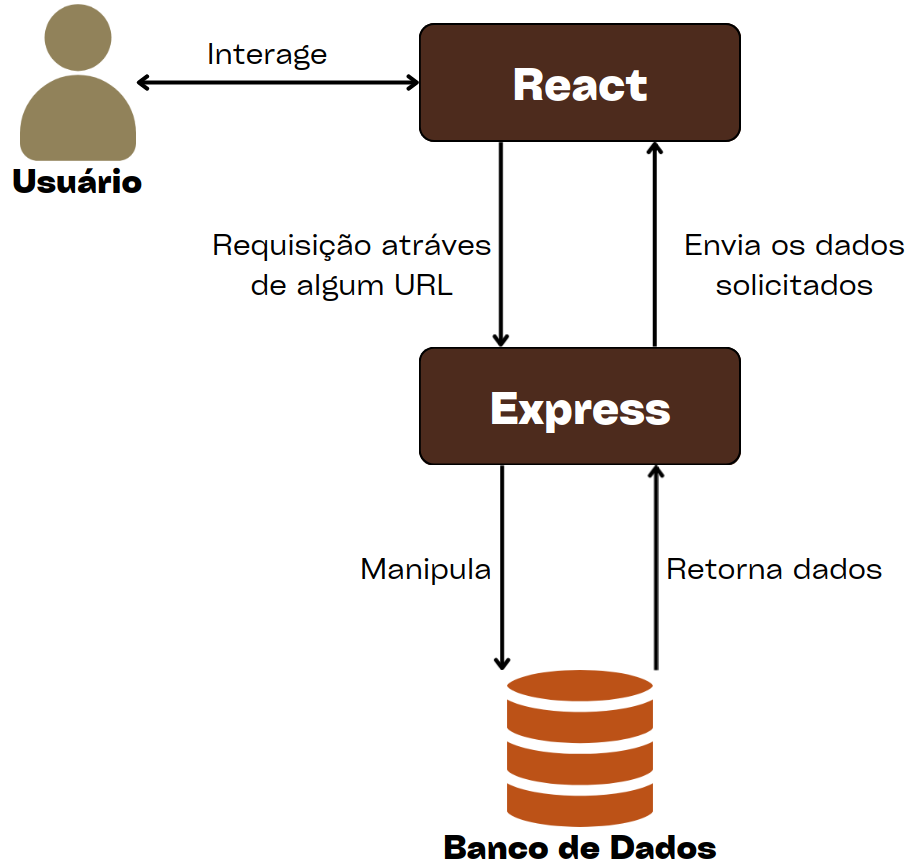
\includegraphics[width=0.5\linewidth]{imagens/architecture.png}
\caption{Arquitetura da aplicação.}
Fonte: própria do autor
\label{fig:architecture}
\end{figure}

\subsubsection{Banco de dados}
O banco de dados foi implementado baseando-se no  diagrama entidade-relacionamento da Figura \ref{fig:er}.

\begin{figure}[hbt!]
\centering
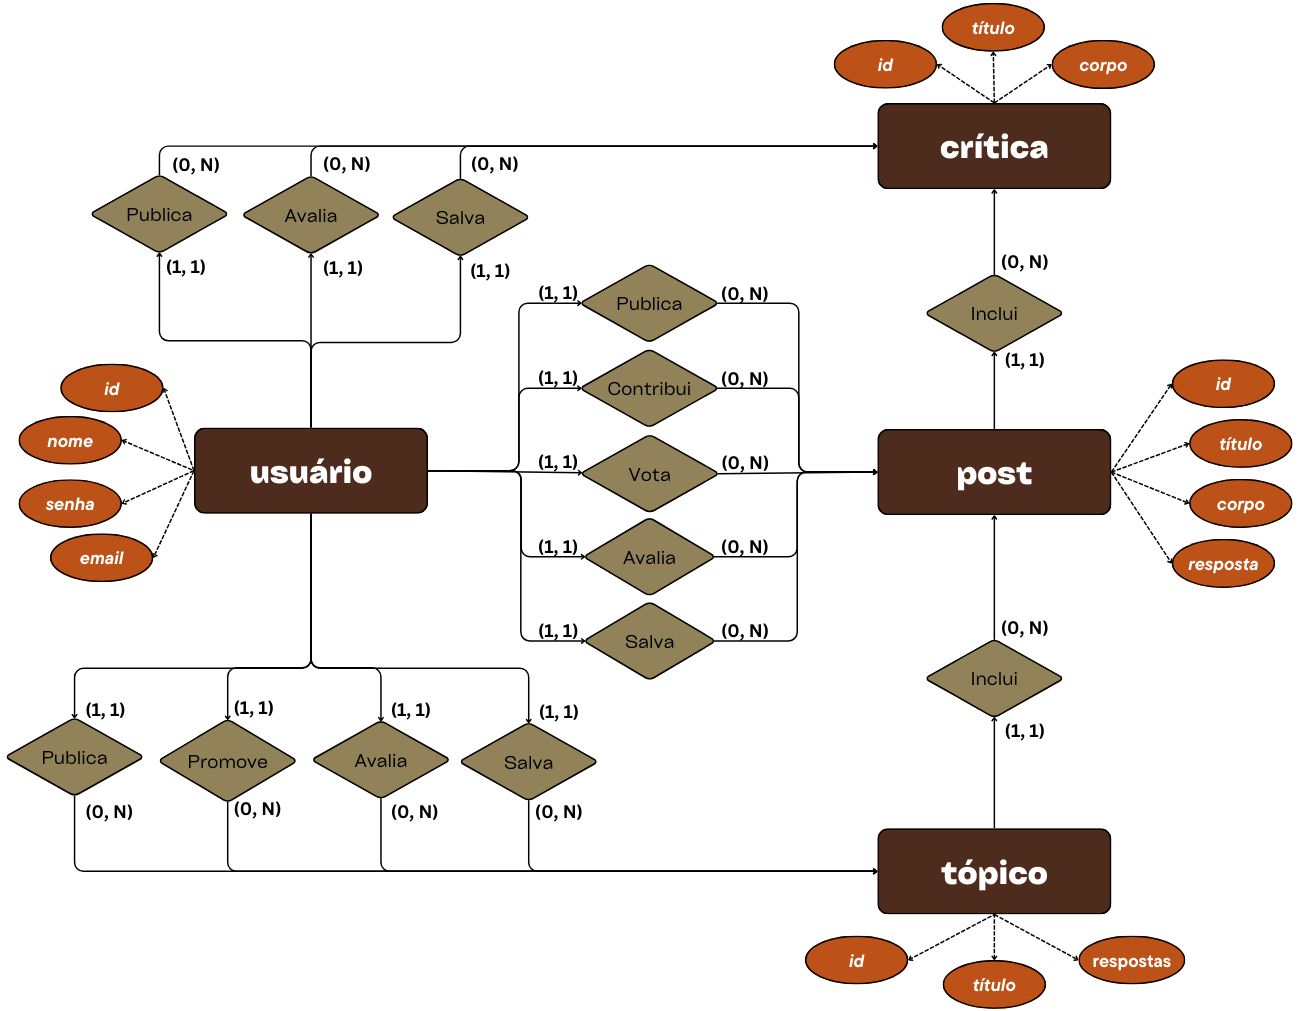
\includegraphics[height=10cm]{imagens/er_diagram.png}
\caption{Diagrama entidade-relacionamento da aplicação.}
Fonte: própria do autor
\label{fig:er}
\end{figure}

As entidades tópico, \textit{post} e crítica foram unificados em uma tabela de conteúdos \textit{contents}, onde a relação entre os conteúdos se dá através de um campo \textit{parent\_id}, que denota o identificador (id) do conteúdo “pai". Para as relações de avaliação, voto, promoção, contribuição e salvamento foram todas consideradas em um tabela de interações \textit{interactions}, na qual o tipo da interação é especificado por uma coluna \textit{type}.

Todos os dados da aplicação foram armazenados utilizando o \textit{PostgreSQL}, com exceção dos dados de corpo dos \textit{posts}, que foram armazenados em arquivos locais gerenciados pelo \textit{Git}, como um SGBD. Cada tópico criado corresponde à uma pasta que contém um repositório \textit{Git}, a partir do qual, para cada \textit{post} criado, cria-se uma nova \textit{branch} correspondente.




\subsection{Interface da aplicação}
A seguir, seguem imagens do design desenvolvido para a aplicação. Como o design depende da existência de conteúdos publicados, fizemos uso de dados \textit{mock}, i.e., dados simulados, para o preenchimento dos campos. Para a paleta de cores utilizada no design da aplicação, foram escolhidas cores visando minimizar a emissão de luz azul, dado que existem evidências que apontam que a luz azul artificial pode prejudicar o sono \cite{blueWorsenSleep}, apesar de que existem outros estudos que ainda apontam inconclusividade em relação a este ponto e outros supostos malefícios da luz azul artificial \cite{blueInconclusive}.


\subsubsection{Principais componentes}
Nesta seção, iremos especificar os principais componentes implementados para compor a interface da aplicação.

\paragraph{\textit{Frame}}

Um \textit{frame}, ou quadro (Figura \ref{fig:frame}), é uma unidade básica de composição, em que outros componentes serão montados em cima. Ele fornece:
\begin{itemize}
    \item \textbf{Botões de voto e avaliação}: São compostos pelas setas e o círculo antes do título, as setas correspondem aos botões de avaliação de relevância, com a seta para cima indicando um conteúdo relevante e, para baixo, um conteúdo não relevante. O botão de voto pode ser usado para múltiplas finalidades que serão descritas nas seções dos próximos componentes;
    \item \textbf{Campo de botões utilitários}: Representado pelos três pontos no canto superior direito, podem ser fornecidos botões com texto e ícones que realizam alguma função quando clicados. Vale ressaltar que no design para \textit{desktop} os ícones são mostrados diretamente, enquanto para \textit{mobile} somente são visíveis ao clicar no ícone de três pontos, abrindo um menu;
    \item \textbf{Campo de corpo}: Pode ser texto ou outros componentes;
    \item \textbf{Campo de rodapé}: Pode ter texto ou uma lista de itens;
    \item \textbf{Campo de título}.
\end{itemize}


\begin{figure}[hbt!]
\centering

\includegraphics[width=0.5\linewidth]{imagens/structure/frame.png}
\caption{Estrutura do \textit{frame}.}
Fonte: própria do autor
\label{fig:frame}
\end{figure}


\paragraph{Tópico}

O tópico contém os seus \textit{posts} de resposta dispostos em ordem decrescente de votos. Os \textit{posts} de cada tópico são expostos em duas partes (Figura \ref{fig:topic}): uma barra com o título do \textit{post} de tamanho proporcional à sua porcentagem de votos e os primeiros 280 caracteres do texto do \textit{post}. \textit{Posts} escritos pelo usuário tem um símbolo de um lápis antes de seu título, e o \textit{post} votado pelo usuário contém um símbolo de uma estrela e uma cor de fundo diferente para a barra. O usuário pode promover o tópico ao clicar no botão de voto, além disso, pode salvar o tópico ao clicar no símbolo de \textit{bookmark} e responder o tópico criando um \textit{post}, ao clicar na seta apontada para esquerda.

\begin{figure}[hbt!]
\centering

\includegraphics[width=0.7\linewidth]{imagens/structure/topic.png}
\caption{Estrutura do tópico.}
Fonte: própria do autor
\label{fig:topic}
\end{figure}



\paragraph{\textit{Post}}

O \textit{post} pode ter, como parte de seu corpo, texto, com as principais funcionalidades de formatação do \textit{Markdown}, além de gráficos e tabelas. O seu botão de voto se destina a realizar o voto no \textit{post corrente} como resposta ao tópico, já os botões utilitários têm as seguintes funções, seguindo da esquerda para a direita:
\begin{itemize}
    \item \textbf{Criar uma \textit{branch}}: Atende ao [RF14], somente visível para usuários que não sejam o autor do post;
    \item \textbf{Realizar \textit{merge} de uma \textit{branch}}: Atende ao [RF17], somente visível para o autor do \textit{post}. Há um contador indicando quantas sugestões foram recebidas;
    \item \textbf{Ocultar/expor críticas};
    \item \textbf{Editar o conteúdo do \textit{post}}: Permite o usuário editar o conteúdo do \textit{post}, quando o usuário terminar, ele pode clicar novamente no ícone e então uma caixa de diálogo será aberta para que ele escolha o que fazer com suas edições. Caso seja o autor, atualiza diretamente o \textit{post}, atendendo ao [RF12], caso não, cria uma nova sugestão de \textit{post}, atendendo ao [RF13];
    \item \textbf{Salvar o \textit{post}}.
\end{itemize}

\begin{figure}[hbt!]
\centering

\includegraphics[width=0.7\linewidth]{imagens/structure/post.png}
\caption{Estrutura do post.}
Fonte: própria do autor
\label{fig:post}
\end{figure}



\paragraph{Crítica}

A crítica não contém um botão de voto, e só tem um botão para salvá-la e um botão para fechá-la. Em seu rodapé consta o nome do autor e a quantidade e divisão dos votos de avaliação de relevância.


\subsubsection{Páginas}

\paragraph{Página de árvore de tópicos}

A tela de visualização de tópicos (Figura \ref{fig:topicTree}) é a tela principal da aplicação e contém até 5 tópicos, sendo o restante acessível por meio do uso de um componente de paginação. Cada tópico exibe os 3 \textit{posts} mais votados, podendo o restante ser visualizado ao entrar na página do tópico através de um clique no título do tópico, ou em reticências que aparecem em seu canto inferior, caso hajam mais de 3 \textit{posts}. Por fim, o conteúdo pode ser ordenado por número de promoções, na aba “promovido" e por ordem de criação, na aba “todos".
\begin{figure}[hbt!]
\centering
\begin{subfigure}{.3\textwidth}
  \centering
  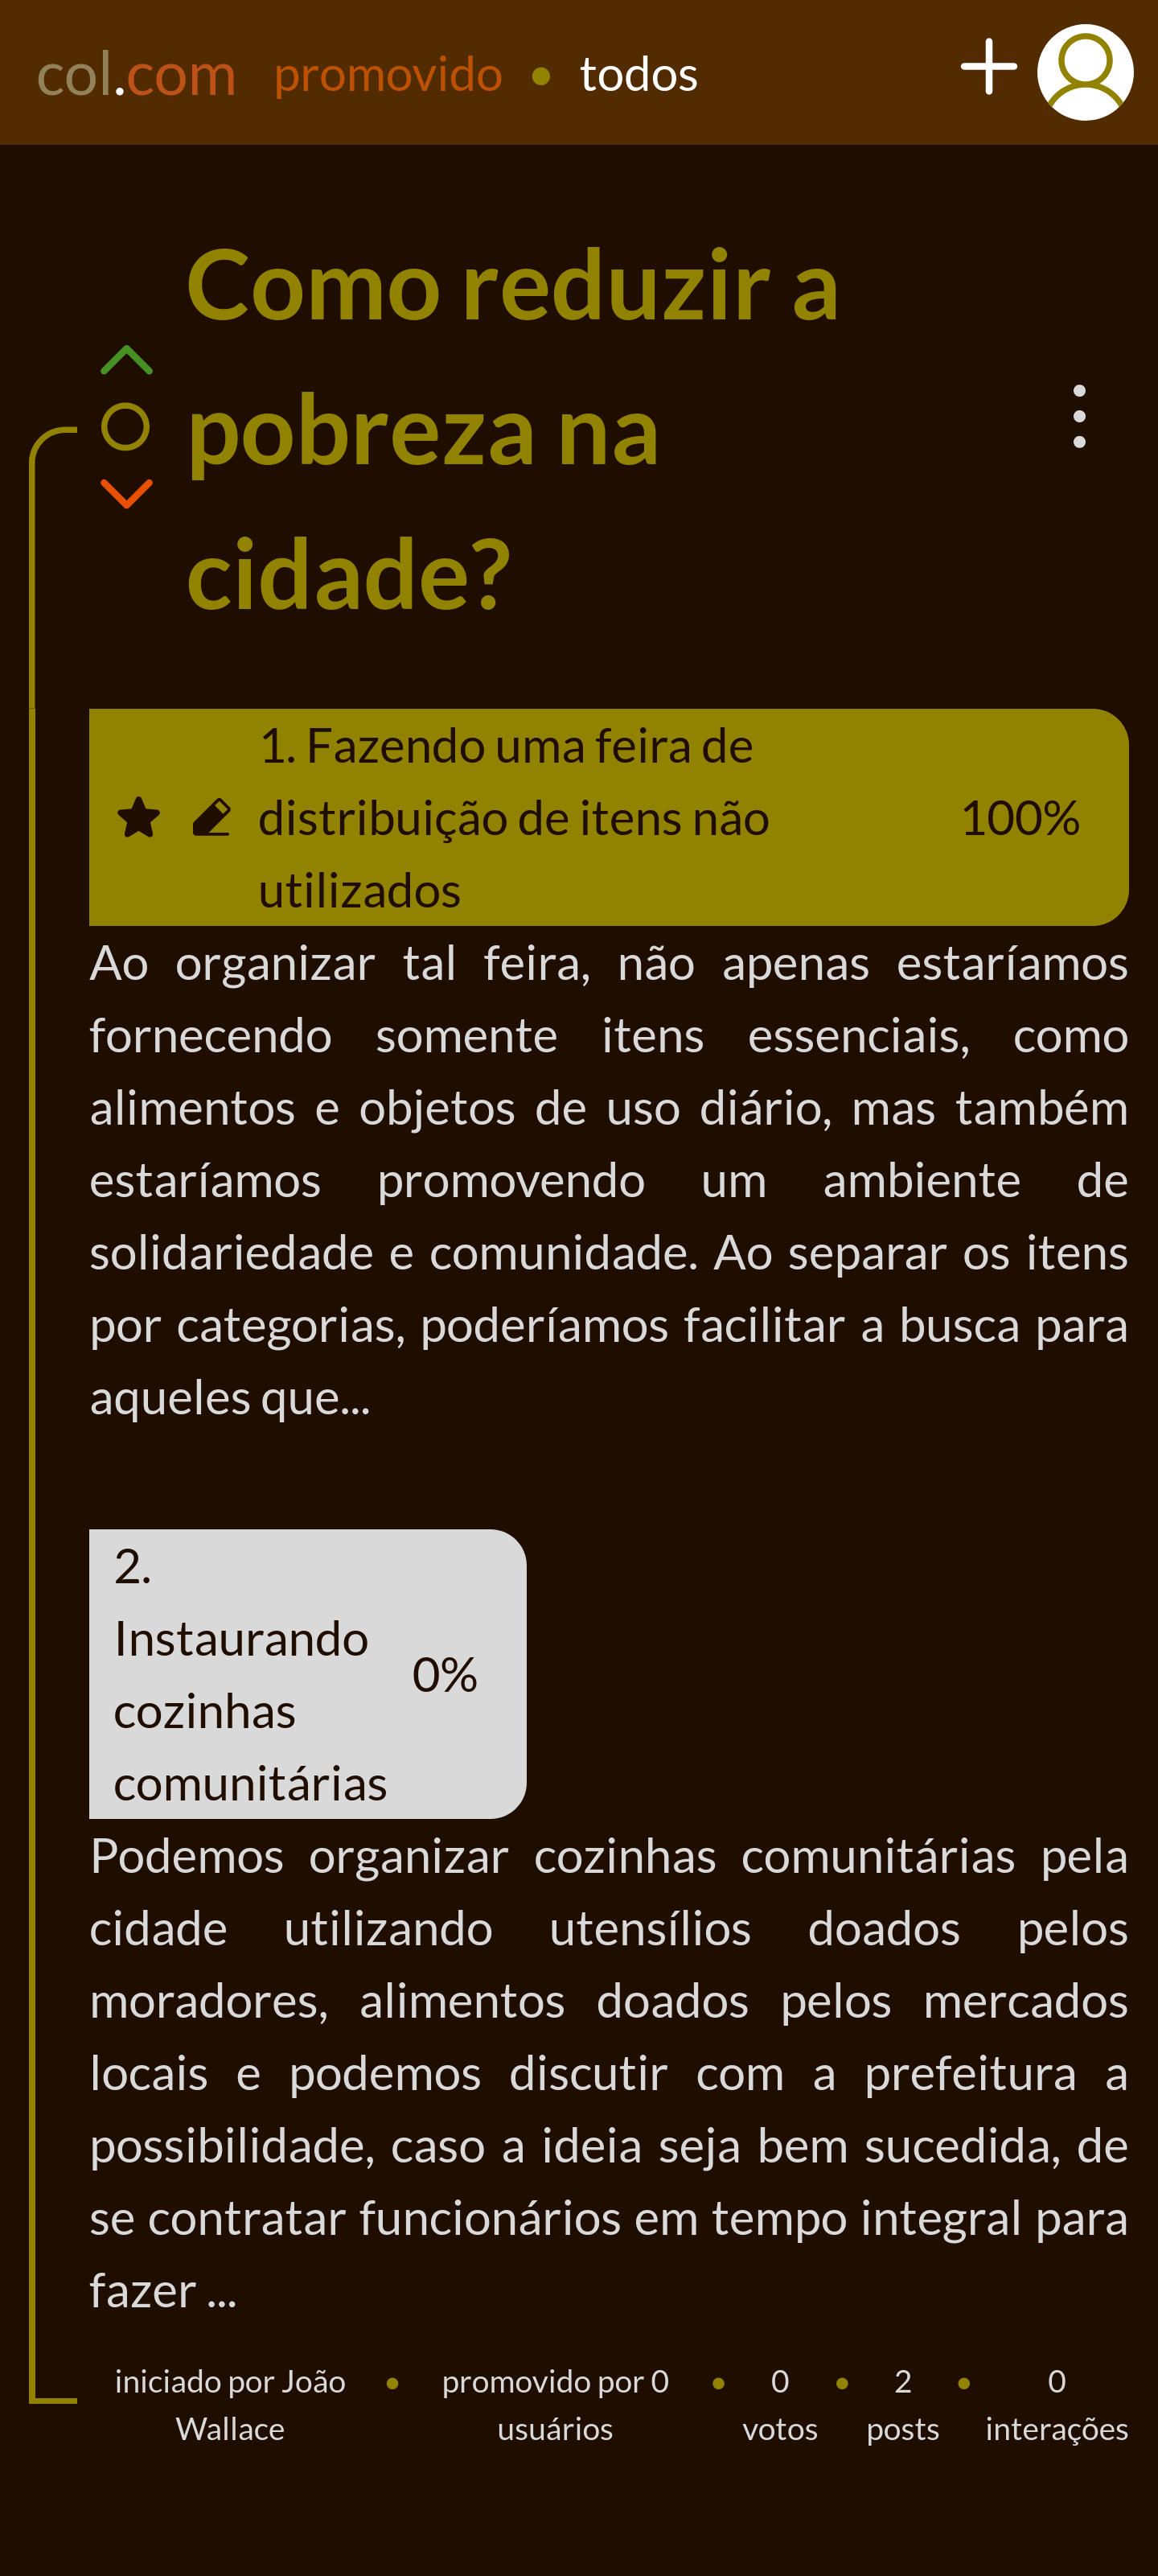
\includegraphics[width=.7\linewidth]{imagens/captures/m_topics.png}
  \caption{Versão mobile}
\end{subfigure}%
\begin{subfigure}{.7\textwidth}
  \centering
  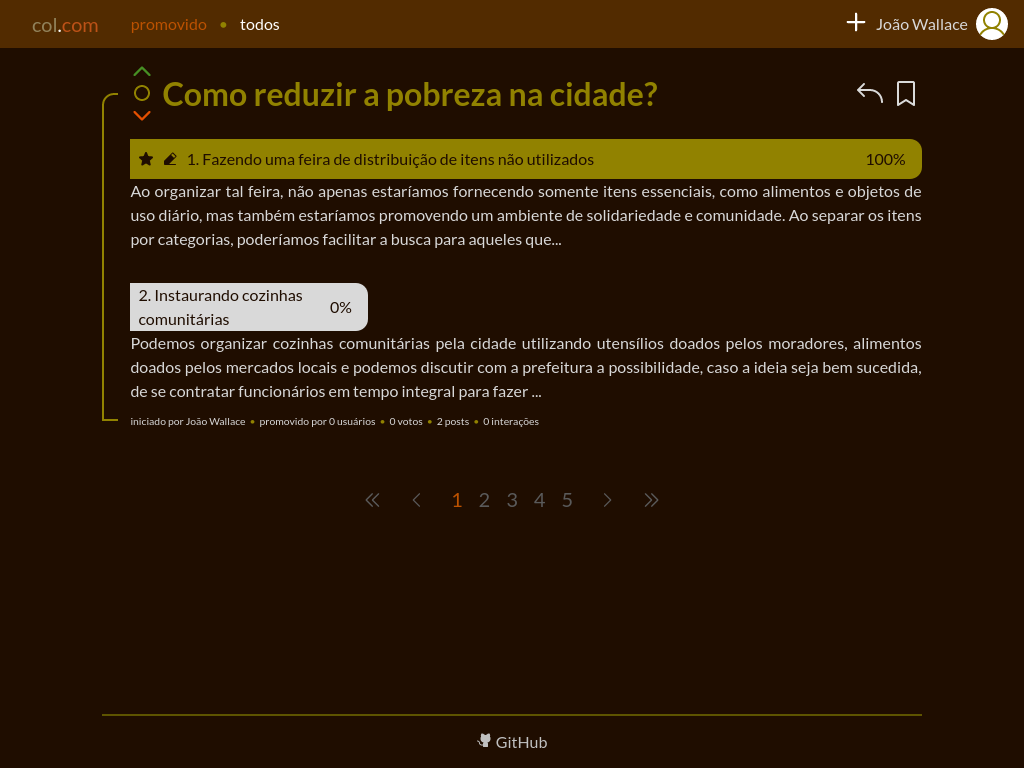
\includegraphics[width=0.9\linewidth]{imagens/captures/topics.png}
  \caption{Versão \textit{desktop}}
\end{subfigure}
\caption{Tela de visualização dos tópicos.}
\label{fig:topicTree}
\end{figure}



\paragraph{Página de tópico}
A página de tópico é semelhante à página de árvore de tópicos, entretanto, só contém um componente de tópico e todos os seus \textit{posts} associados.

% \newpage

\paragraph{Página de \textit{post}}

Como exposto na Figura \ref{fig:postPage}, a tela de um \textit{post} é composta por três elementos, sendo eles de cima para baixo: um \textit{link} para seu tópico pai, uma barra \textit{slider}, para seleção da versão e o \textit{post} em si. Através da tela de \textit{post}, também é possível visualizar as críticas realizadas ao \textit{post} em cada uma de suas versões, como demonstrado na Figura \ref{fig:postCritique}. Críticas feitas em trechos que se sobrepõem são unidas em um mesmo bloco que, ao ser clicado, exibe a lista de todas as críticas contidas nele; para se identificar o trecho específico de uma crítica contida em um bloco, o usuário pode clicar em seu título, assim marcando o trecho condizente.


\begin{figure}[hbt!]
\centering
\begin{subfigure}{.3\textwidth}
  \centering
  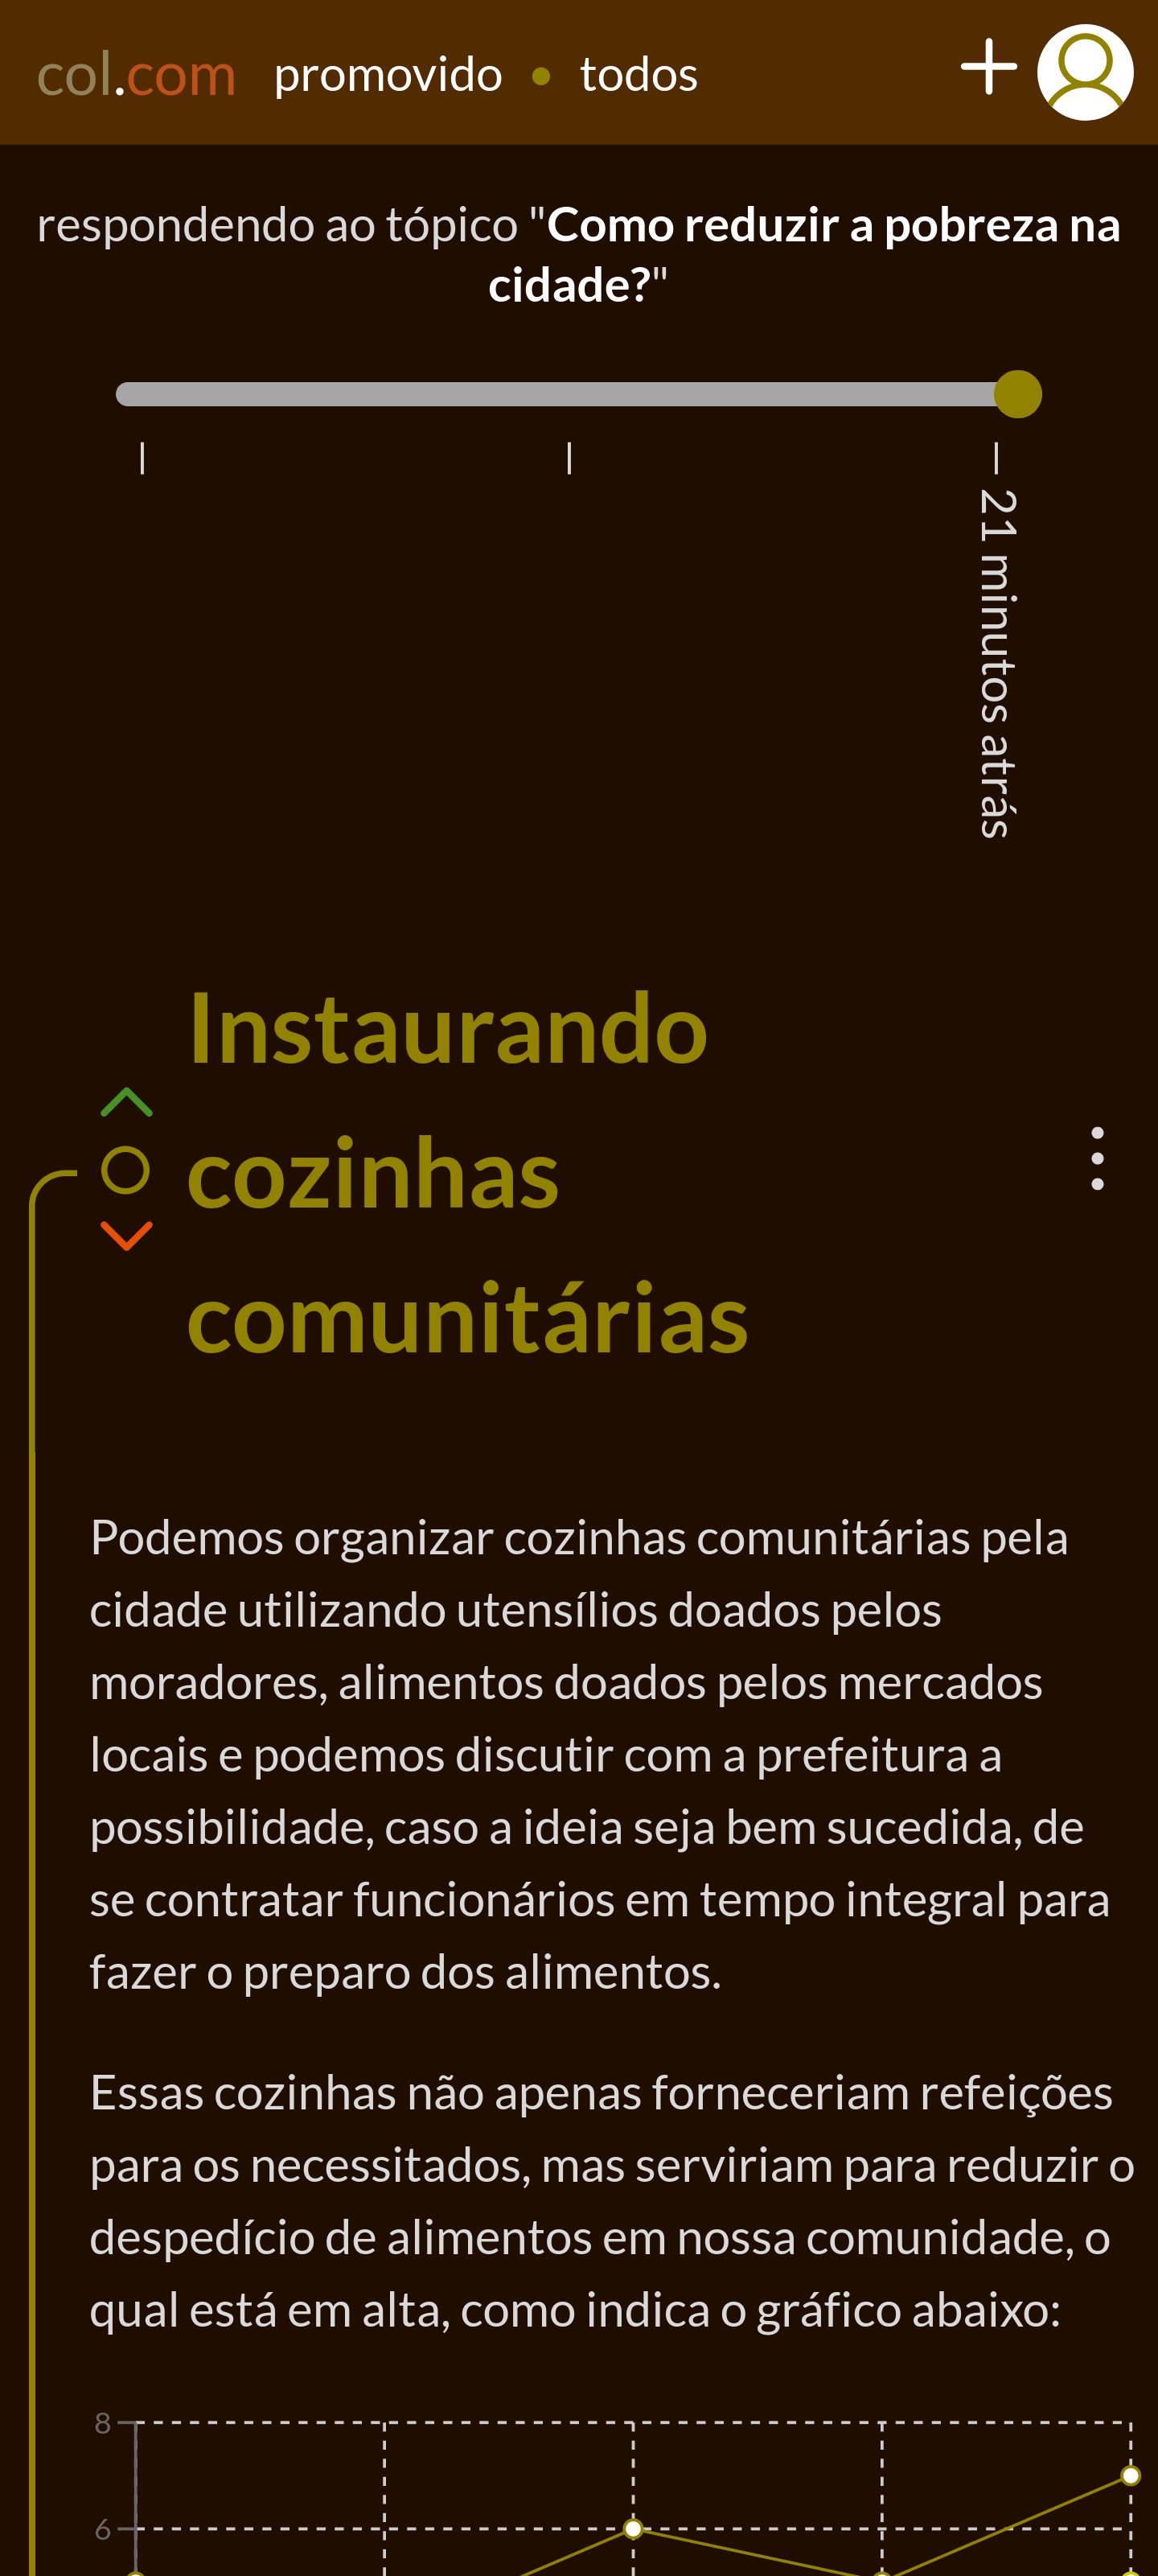
\includegraphics[width=.68\linewidth]{imagens/captures/m_post.png}
  \caption{Versão mobile}
\end{subfigure}%
\begin{subfigure}{.7\textwidth}
  \centering
  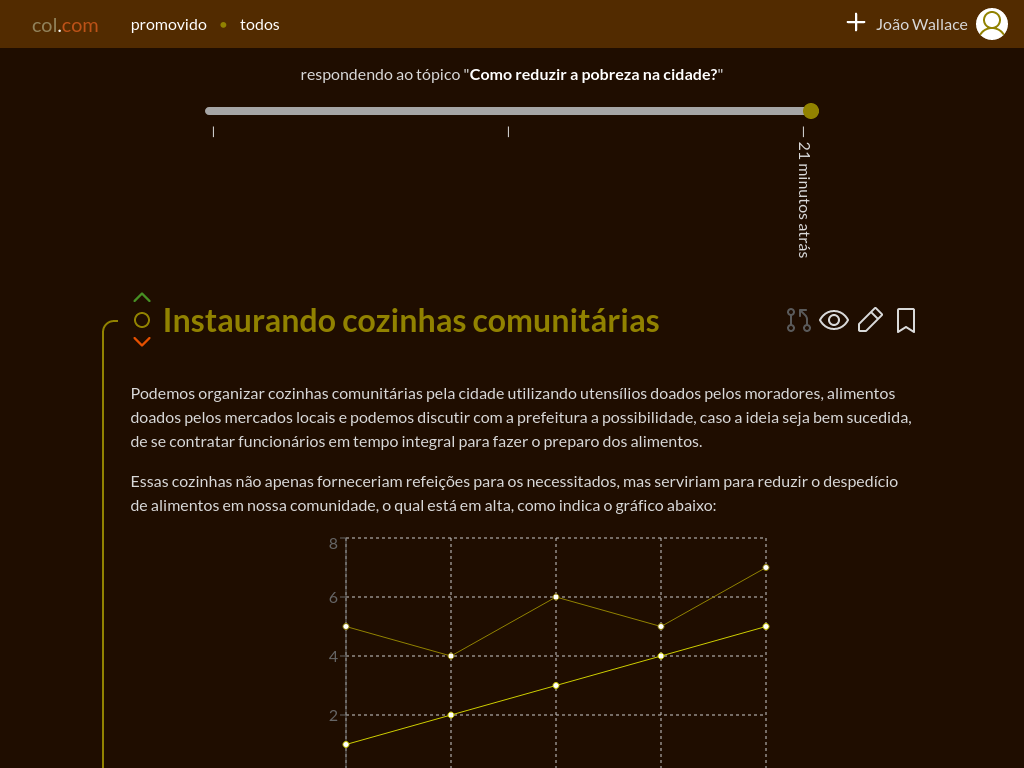
\includegraphics[width=0.87\linewidth]{imagens/captures/post.png}
  \caption{Versão desktop}
\end{subfigure}
\caption{Tela de visualização do \textit{post}.}
\label{fig:postPage}
\end{figure}


\begin{figure}[hbt!]
\centering
\begin{subfigure}{.3\textwidth}
  \centering
  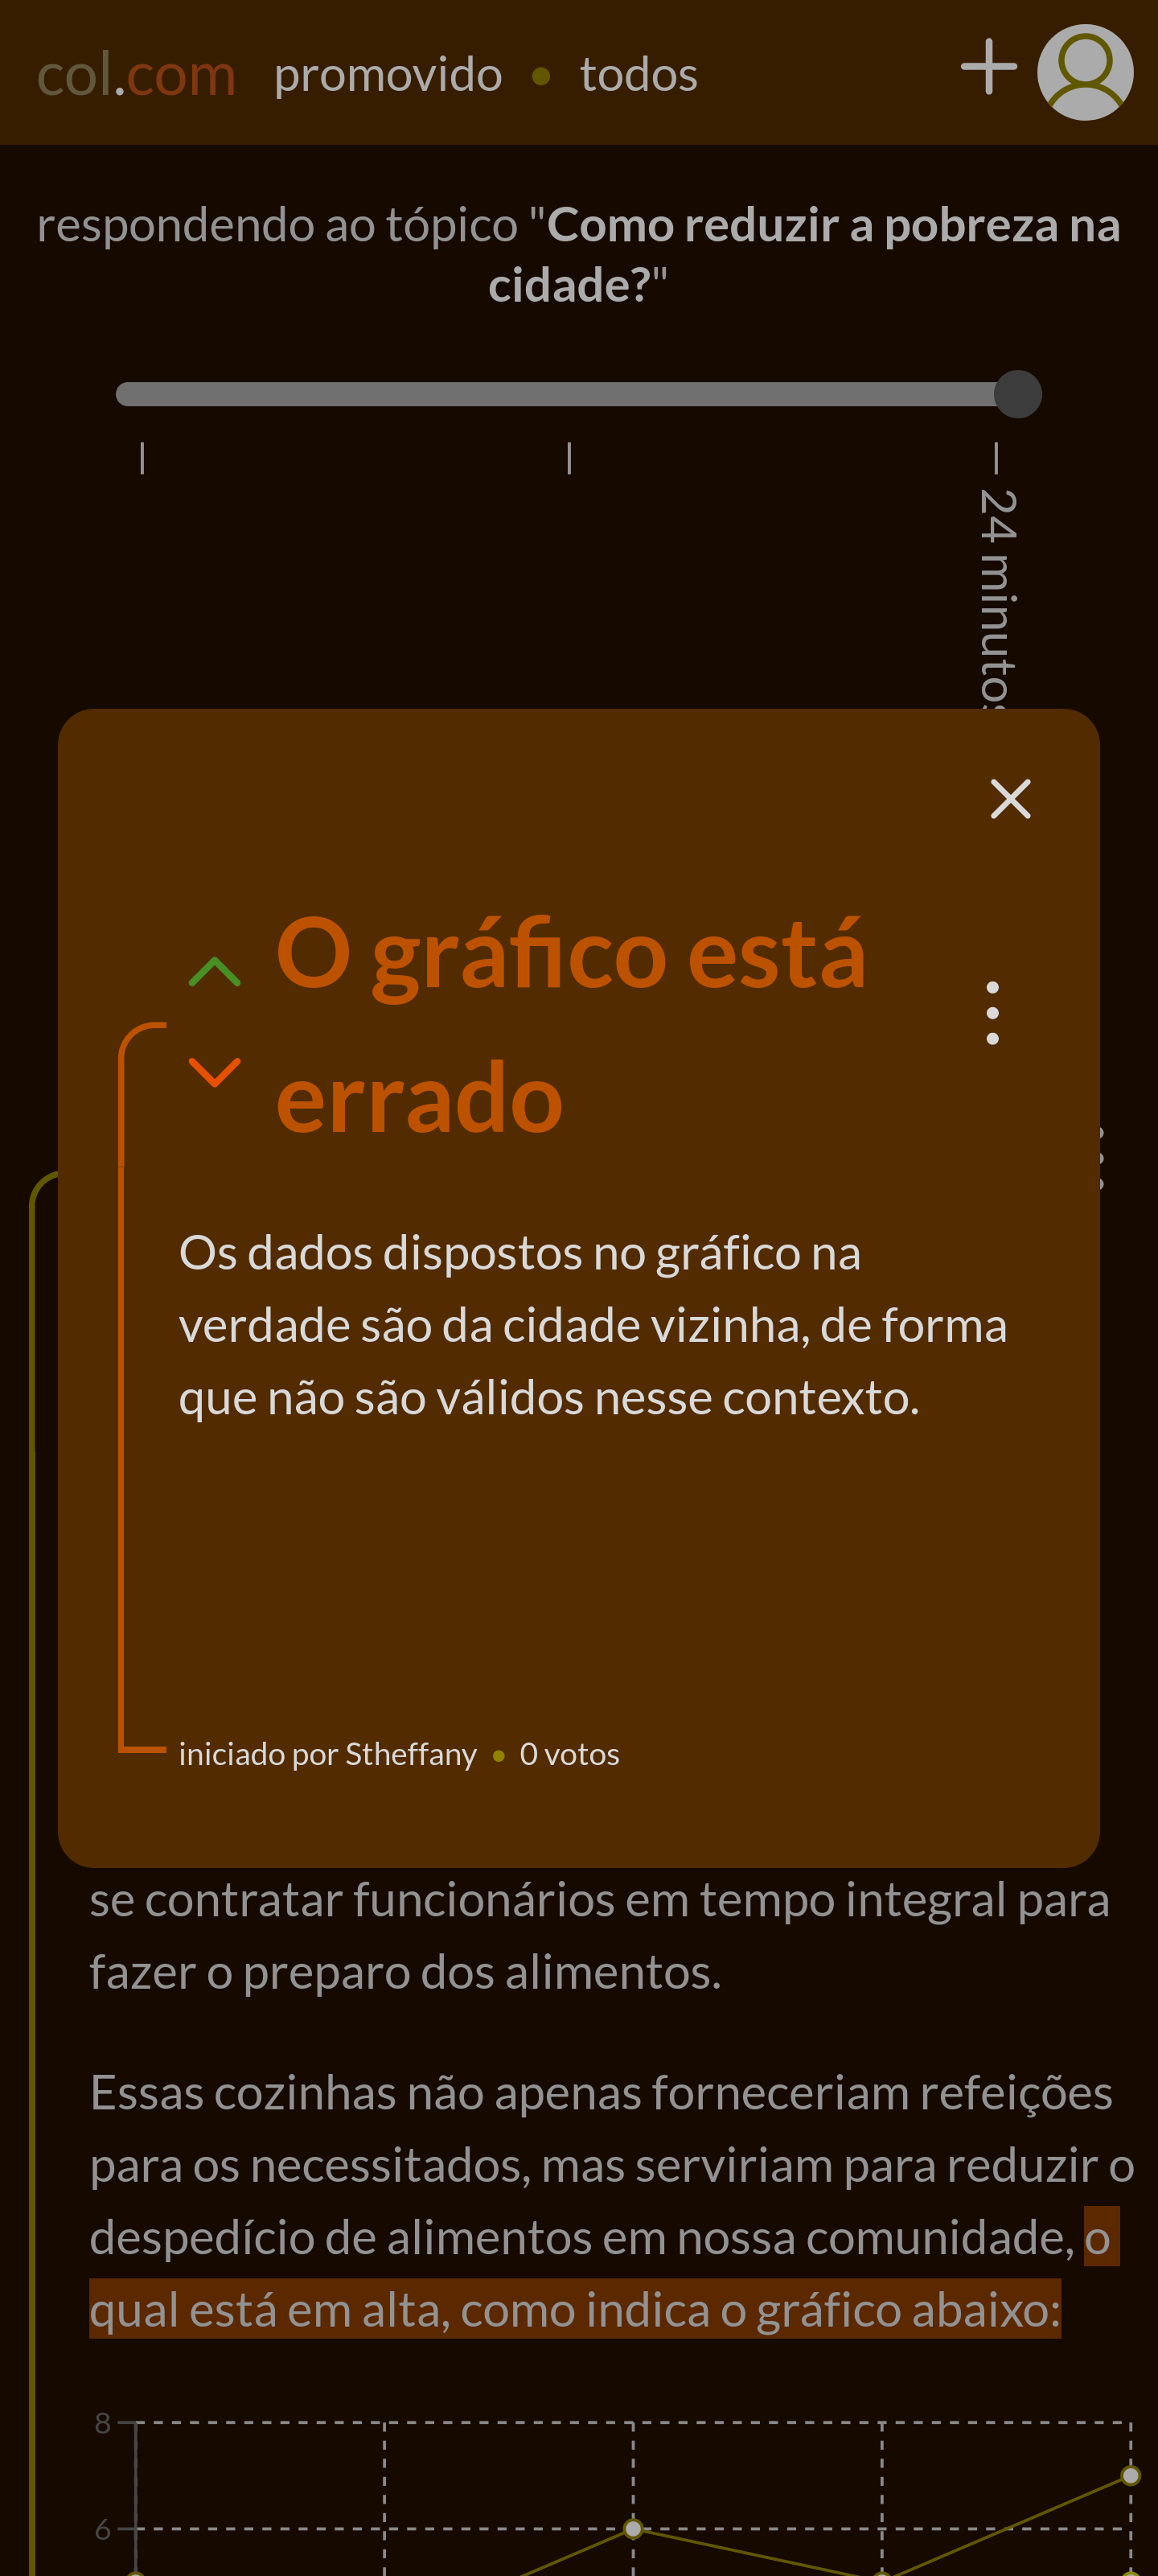
\includegraphics[width=.68\linewidth]{imagens/captures/m_post_critique.png}
  \caption{Versão mobile}
\end{subfigure}%
\begin{subfigure}{.7\textwidth}
  \centering
  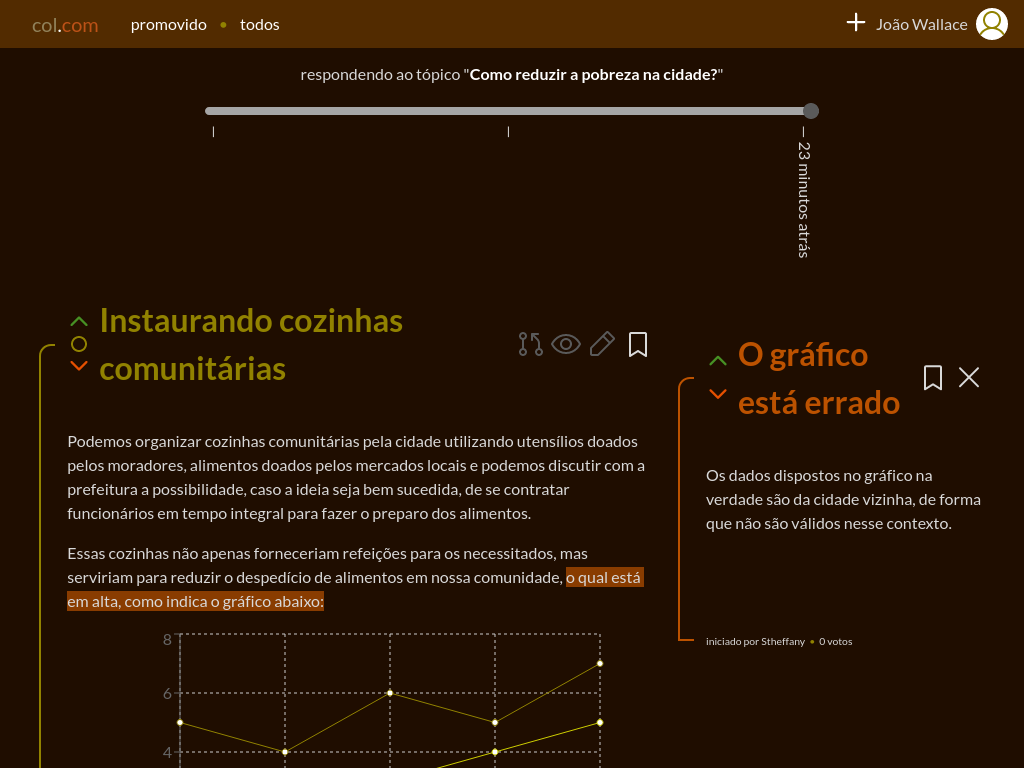
\includegraphics[width=0.87\linewidth]{imagens/captures/post_critique.png}
  \caption{Versão desktop}
\end{subfigure}
\caption{Tela de um post com uma crítica sendo visualizada.}
\label{fig:postCritique}
\end{figure}


\paragraph{Página de \textit{login} e cadastro}
O \textit{login} e cadastro do usuário são realizados na mesma página, esta exposta na Figura \ref{fig:login}, sendo possível alternar entre duas operações ao clicar no texto “crie uma agora!", para se direcionar ao cadastro, e “entre agora!" para o \textit{login}. O formulário de cadastro é exposto na Figura \ref{fig:signup}.

\begin{figure}[hbt!]
\centering
\begin{subfigure}{.3\textwidth}
  \centering
  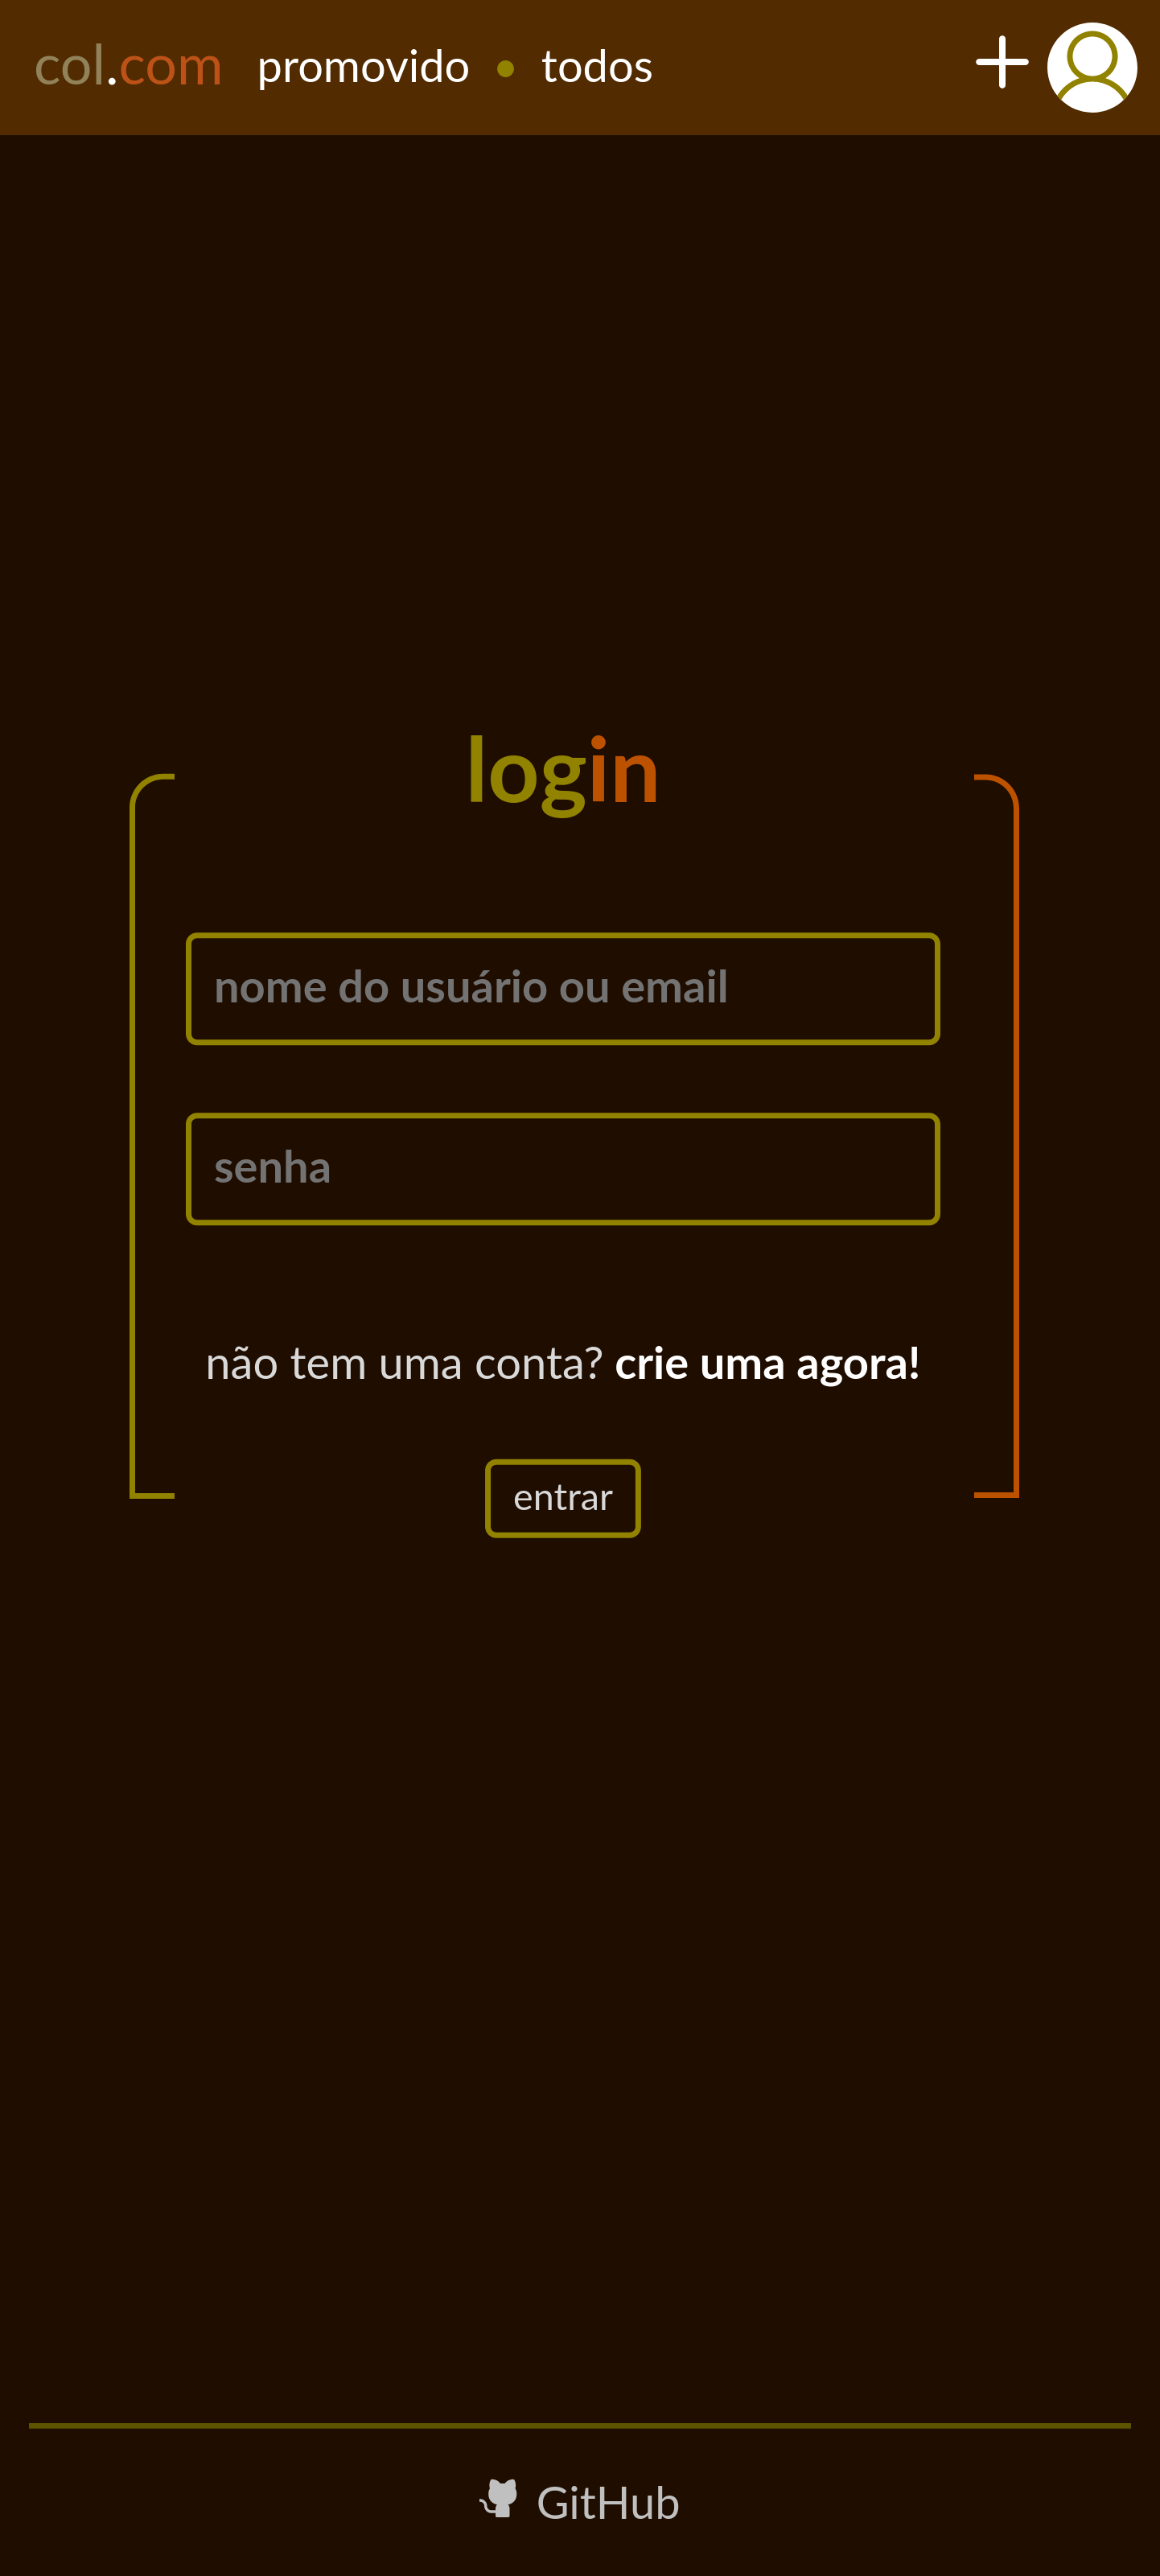
\includegraphics[width=.66\linewidth]{imagens/captures/m_login.png}
  \caption{Versão mobile}
\end{subfigure}%
\begin{subfigure}{.7\textwidth}
  \centering
  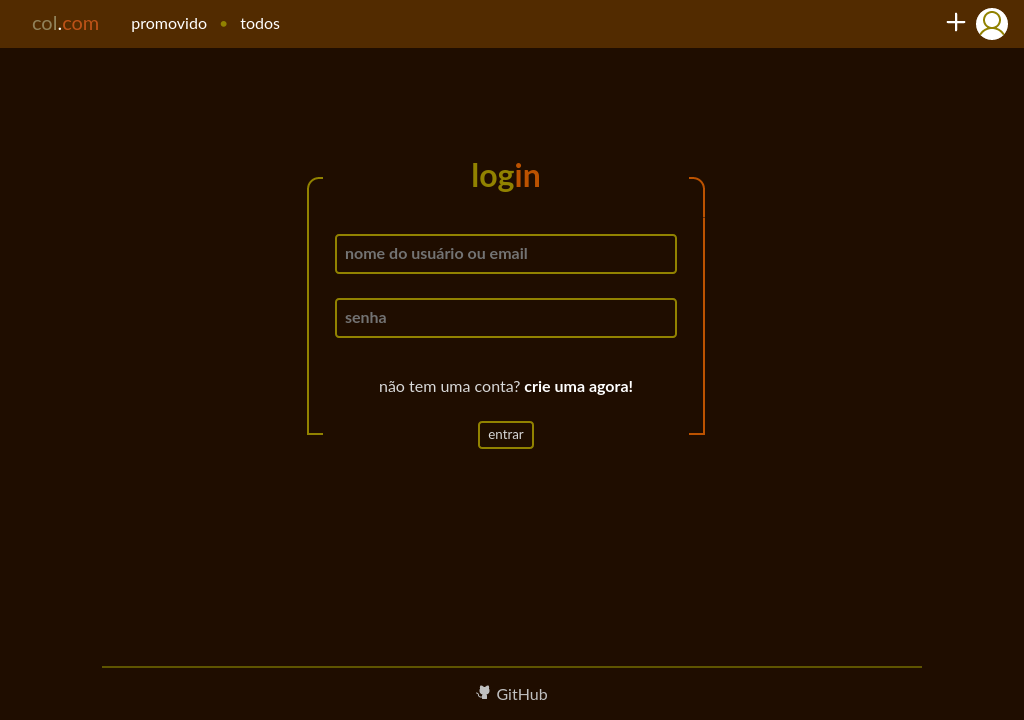
\includegraphics[width=0.9\linewidth]{imagens/captures/login.png}
  \caption{Versão desktop}
\end{subfigure}
\caption{Tela de \textit{login} e cadastro.}
\label{fig:login}
\end{figure}

\begin{figure}[hbt!]
\centering
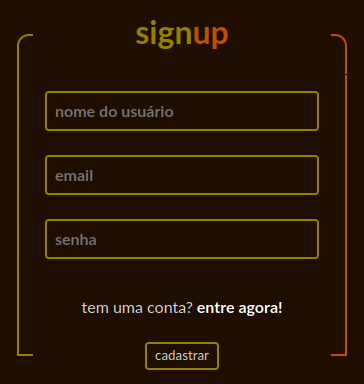
\includegraphics[width=0.275\linewidth]{imagens/captures/signup.png}
\caption{Formulário de cadastro.}
\label{fig:signup}
\end{figure}

\paragraph{Página de conteúdos salvos}
A página de conteúdos salvos contém todos os tópicos, \textit{posts} e críticas salvos pelo usuário, dispostos de maneira similar à árvore de tópicos.

\paragraph{Página de edição de texto}
Na página de edição de texto, o usuário pode escrever um \textit{post}, informando um título e fornecendo um corpo. O corpo do \textit{post} pode conter texto, com estilizações do \textit{Markdown}, tabelas e gráficos.

\clearpage

\section{APRESENTAÇÃO E ANÁLISE DOS RESULTADOS}
% Toda pesquisa deve apresentar uma análise sobre a investigação que foi realizada através da metodologia que foi aplicada. Nesta sessão é interessante inserir tabelas, gráficos, imagens que mostrem os resultados, análise de dados coletados, etc.

% É interessante que nessa sessão o autor compare os seus resultados com os resultados de outros trabalhos existentes. Essa comparação aumenta a qualidade do trabalho e demonstra a relevância do mesmo. 

% Nesta sessão o autor pode/deve incluir as contribuições científicas desenvolvidas tais como artigos, patentes, livros e outras contibuições que foram publicadas ou estão em fase de publicação e que são parte do trabalho.

Este capítulo é destinado para a exposição dos resultados, os quais foram obtidos através do plano de testes, detalhado a seguir.

\subsection{Plano de testes}
O objetivo do plano de testes é permitir a identificação de eventuais problemas de implementação na aplicação, de modo a assegurar o funcionamento esperado da plataforma. Para tal, será realizada uma navegação por todas as principais funcionalidades da aplicação, partindo do cadastro de usuário até a publicação de conteúdos.

% Os testes foram realizados por meio de uma instância hospedada localmente em uma máquina dedicada com Ubuntu Server 22.04 LTS.
Para efetuar tais testes, tanto a aplicação \textit{front-end} como a \textit{back-end} foram hospedadas localmente em uma máquina dedicada com \textit{Ubuntu Server} 22.04 LTS. A partir desta, o sistema foi acessado de diferentes dispositivos, como \textit{desktops}, \textit{notebooks} e \textit{smartphones}, e usou-se  diferentes navegadores, como \textit{Google Chrome}, \textit{Firefox} e \textit{Safari}, a fim de garantir a disposição correta da aplicação em diferentes combinações de tecnologias.

Infelizmente, os testes foram conduzidos exclusivamente pelo autor do presente trabalho, dado que não foi possível realizar testes com usuários reais antes da data de apresentação do mesmo.

\subsection{Casos de teste}
A seguir, Nas Tabelas 1-13, serão descritos os casos de teste considerados de maior importância para o fluxo principal de funcionamento da plataforma.

\begin{table}[hbt!]
    \centering
    \begin{tabularx}{0.9\textwidth}{l|X}
    \hline
    \textbf {Título} & [T01] Cadastrar usuário \\\hline
    \textbf {Descrição} & Testa-se o cadastro de um usuário não registrado. Refere-se ao [RF01]. \\ \hline
    \textbf {Passos do teste} & O usuário preenche os campos de nome de usuário, email e senha e clica em “cadastrar". \\ \hline
    \textbf {Resultado esperado} & O cadastro do usuário deve ser criado no banco de dados, e o usuário dever ser redirecionado para a tela de login. \\ \hline
    \textbf {Resultado obtido} & Sucesso. \\ \hline
    \end{tabularx}
    \caption{Caso de teste [T01].}
\end{table}


\begin{table}[hbt!]
    \centering
    \begin{tabularx}{0.9\textwidth}{l|X}
    \hline
    \textbf {Título} & [T02] Logar usuário \\\hline
    \textbf {Descrição} & Testa-se a realização do \textit{login} de um usuário. Refere-se ao [RF02]. \\ \hline
    \textbf {Passos do teste} & O usuário preenche os campos de nome de usuário/email e senha e clica em “entrar". \\ \hline
    \textbf {Resultado esperado} & O usuário deve ser redirecionado para a tela de “promovido" com seus dados carregados. \\ \hline
    \textbf {Resultado obtido} & Sucesso. \\ \hline
    \end{tabularx}
    \caption{Caso de teste [T02].}
\end{table}

\begin{table}[hbt!]
    \centering
    \begin{tabularx}{0.9\textwidth}{l|X}
    \hline
    \textbf {Título} & [T03] Criar um tópico\\\hline
    \textbf {Descrição} & Testa-se a criação de um tópico. Refere-se ao [RF05] \\ \hline
    \textbf {Passos do teste} & O usuário clica no botão com um “+" na barra de navegação, abrindo um modal, o usuário então preenche os campos de título, marca se deseja que outros usuários possam submeter múltiplos posts e descreve as possíveis respostas, caso já as tenha previamente. \\ \hline
    \textbf {Resultado esperado}& O tópico é criado no banco de dados e o usuário é redirecionado para a página do tópico. \\ \hline
    \textbf {Resultado obtido} & Sucesso. \\ \hline
    \end{tabularx}
    \caption{Caso de teste [T03].}
\end{table}


\begin{table}[hbt!]
    \centering
    \begin{tabularx}{0.9\textwidth}{l|X}
    \hline
    \textbf {Título} & [T04] Avaliar um tópico como relevante \\\hline
    \textbf {Descrição} & Testa-se os botões de avaliação “relevante" e “não relevante" em um tópico. Refere-se ao [RF03]. \\ \hline
    \textbf {Passos do teste} & O usuário clica nas setas de avaliação de um tópico, primeiro para definir como “não relevante" e depois para “relevante". \\ \hline
    \textbf {Resultado esperado}& As setas aparecem preenchidas quando o usuários as clica, gerando um registro de interação correspondente no banco de dados. \\ \hline
    \textbf {Resultado obtido} & Sucesso. \\ \hline
    \end{tabularx}
    \caption{Caso de teste [T04].}
\end{table}

\begin{table}[hbt!]
    \centering
    \begin{tabularx}{0.9\textwidth}{l|X}
    \hline
    \textbf {Título} & [T05] Salvar um tópico \\\hline
    \textbf {Descrição} & Testa-se o botão de salvar de um tópico. Refere-se ao [RF04]. \\ \hline
    \textbf {Passos do teste} & O usuário clica no botão de salvar de um tópico. \\ \hline
    \textbf {Resultado esperado}& O ícone do botão se torna preenchido e uma interação de salvamento é criada no banco de dados. \\ \hline
    \textbf {Resultado obtido} & Sucesso. \\ \hline
    \end{tabularx}
    \caption{Caso de teste [T05].}
\end{table}

\begin{table}[hbt!]
    \centering
    \begin{tabularx}{0.9\textwidth}{l|X}
    \hline
    \textbf {Título} & [T06] Promover um tópico \\\hline
    \textbf {Descrição} & Testa-se o botão de promoção de um tópico. Refere-se ao [RF06]. \\ \hline
    \textbf {Passos do teste} & O usuário clica no botão de promover de um tópico. \\ \hline
    \textbf {Resultado esperado}& O ícone do botão de promover se torna preenchido e uma interação de promoção vigente até o fim do dia é criada no \textit{back-end}. \\ \hline
    \textbf {Resultado obtido} & Sucesso. \\ \hline
    \end{tabularx}
    \caption{Caso de teste [T06].}
\end{table}

\begin{table}[hbt!]
    \centering
    \begin{tabularx}{0.9\textwidth}{l|X}
    \hline
    \textbf {Título} & [T07] Criar um \textit{post} em resposta a um tópico \\\hline
    \textbf {Descrição} & Testa-se o fluxo de criação de um \textit{post} em resposta a um tópico. Refere-se aos [RF09] e [RF10]. \\ \hline
    \textbf {Passos do teste} & O usuário clica no botão de responder de um tópico, e, após ser redirecionado à pagina de escrita, preenche o campo de título e resposta, caso haja opções de resposta, e digita um texto contendo todas as funcionalidades do editor de texto, e então clica no botão “publicar". \\ \hline
    \textbf {Resultado esperado}& O \textit{post} é criado no \textit{back-end} e o usuário é redirecionado para a página do textit{post}. \\ \hline
    \textbf {Resultado obtido} & Sucesso. \\ \hline
    \end{tabularx}
    \caption{Caso de teste [T07].}
\end{table}

\begin{table}[hbt!]
    \centering
    \begin{tabularx}{0.9\textwidth}{l|X}
    \hline
    \textbf {Título} & [T08] Editar um \textit{post} \\\hline
    \textbf {Descrição} & Testa-se a edição de um \textit{post}. Refere-se ao [RF12]. \\ \hline
    \textbf {Passos do teste} & O usuário clica no botão de edição de um tópico, então faz alterações no texto do \textit{post} através do editor de texto, e após de finalizado clica novamente no símbolo de edição, abrindo um modal, por fim o usuário preenche o campo de resumo das alterações e clica no botão “enviar". \\ \hline
    \textbf {Resultado esperado}& O \textit{slider} de versões registra a nova versão e a edição é enviada para o \textit{back-end}, que cria um novo \textit{commit} no banco de dados. \\ \hline
    \textbf {Resultado obtido} & Sucesso. \\ \hline
    \end{tabularx}
    \caption{Caso de teste [T08].}
\end{table}

\begin{table}[hbt!]
    \centering
    \begin{tabularx}{0.9\textwidth}{l|X}
    \hline
    \textbf {Título} & [T09] Criar uma sugestão de edição para um \textit{post} \\\hline
    \textbf {Descrição} & Testa-se a criação de uma sugestão de edição para um \textit{post}. Refere-se ao [RF13]. \\ \hline
    \textbf {Passos do teste} & Loga-se em uma conta diferente da usada para a criação do \textit{post} e segue-se o exato mesmo passo a passo do [T08]. \\ \hline
    \textbf {Resultado esperado}& São criados uma nova interação de sugestão e um \textit{commit} em uma nova \textit{branch} no banco de dados. \\ \hline
    \textbf {Resultado obtido} & Sucesso. \\ \hline
    \end{tabularx}
    \caption{Caso de teste [T09].}
\end{table}

\begin{table}[hbt!]
    \centering
    \begin{tabularx}{0.9\textwidth}{l|X}
    \hline
    \textbf {Título} & [T10] Criar um “ramo” de uma versão específica de um \textit{post} \\\hline
    \textbf {Descrição} & Testa-se a criação de um “ramo” de uma versão específica de um \textit{post}. Refere-se ao [RF14]. \\ \hline
    \textbf {Passos do teste} & Loga-se em uma conta diferente da usada para a criação do \textit{post} e o usuário clica no botão de clonar do \textit{post}, abrindo um modal, o usuário então preenche o campo “título da cópia" e clica em “clonar".  \\ \hline
    \textbf {Resultado esperado}& É criado uma nova \textit{branch} pertencente ao usuário no banco de dados, por fim o usuário é redirecionado para a página do \textit{post} criado. \\ \hline
    \textbf {Resultado obtido} & Sucesso. \\ \hline
    \end{tabularx}
    \caption{Caso de teste [T10].}
\end{table}

\begin{table}[hbt!]
    \centering
    \begin{tabularx}{0.9\textwidth}{l|X}
    \hline
    \textbf {Título} & [T11] Acatar sugestão de edição de um \textit{post} \\\hline
    \textbf {Descrição} & Testa-se o acatamento de uma sugestão de edição em um \textit{post}. Refere-se aos [RF16] e [RF17]. \\ \hline
    \textbf {Passos do teste} & O usuário autor do \textit{post} clica no botão de incorporar sugestões do \textit{post}, abrindo um modal, então o usuário clica no título de uma das sugestões sendo redirecionado ao \textit{post} com a edição sugerida, então clica no botão de aceitar sugestão. \\ \hline
    \textbf {Resultado esperado} & É realizado o \textit{merge} da \textit{branch} do autor do \textit{post} e do autor da sugestão no banco de dados, então o usuário é redirecionado para a página do post refletindo as alterações. \\ \hline
    \textbf {Resultado obtido} & Sucesso. \\ \hline
    \end{tabularx}
    \caption{Caso de teste [T11].}
\end{table}

\clearpage

\begin{table}[hbt!]
    \centering
    \begin{tabularx}{0.9\textwidth}{l|X}
    \hline
    \textbf {Título} & [T12] Realizar uma crítica em um \textit{post} \\\hline
    \textbf {Descrição} & Testa-se a realização de uma crítica em um \textit{post}. Refere-se ao [RF19]. \\ \hline
    \textbf {Passos do teste} & O usuário seleciona um trecho do texto do \textit{post}, e então clica no botão “criticar", abrindo um \textit{frame} de crítica, o usuário então preenche o título e corpo da crítica e clica no botão de confirmar. \\ \hline
    \textbf {Resultado esperado} & O trecho criticado é sublinhado e é criado um registro da crítica no banco de dados. \\ \hline
    \textbf {Resultado obtido} & Sucesso. \\ \hline
    \end{tabularx}
    \caption{Caso de teste [T12].}
\end{table}

% \begin{table}[hbt!]
%     \centering
%     \begin{tabularx}{0.9\textwidth}{l|X}
%     \hline
%     \textbf {Título} & [T13] Cadastrar um usuário inválido \\\hline
%     \textbf {Descrição} & Testa-se a rejeição do cadastro de usuários inválidos. \\ \hline
%     \textbf {Passos do teste} & . \\ \hline
%     \textbf {Resultado esperado} & . \\ \hline
%     \textbf {Resultado obtido} & Falha. \\ \hline
%     \end{tabularx}
%     \caption{Caso de teste [T13].}
% \end{table}

\subsection{Comparativo com outras plataformas}
Nesta seção, faremos um comparativo de funcionalidades entre a nossa solução e outras propostas semelhantes, já estabelecidas

%% \subsubsection{Plataformas de democracia digital}
\subsubsection{\textit{Pol.is}}
A premissa principal do \textit{Polis} é coletar um grande número de amostras de opiniões de seus usuários e aplicar uma redução de dimensionalidade, através de uma Análise de Componentes Principais (do inglês, \textit{Principal Components Analysis} - PCA), e então aplicar um algoritmo de clusterização, em seu caso um \textit{K-means}, para agrupar os participantes em grupos de opiniões semelhantes, e, então, encontrar pontos comuns entre os diferentes grupos e os pontos que melhor representam cada grupo, visando estimular o diálogo e compreensão mútua entre tais grupos e eventualmente fomentar o consenso.

Nossa plataforma se diferencia ao possibilitar que os participantes criem conjuntamente respostas cada vez mais complexas e completas, ao fazer uso das propriedades evolutivas do SCV. Através de um engajamento contínuo e competição entre as diversas respostas espera-se que os usuários cheguem em um conjunto de respostas que representem melhor cada grupo. Enquanto o \textit{Polis} objetiva ao fim obter várias frases curtas que representem a opinião de seus usuários, nós pretendemos que os usuários criem as respostas mais completas, que representem suas opiniões. Outro ponto de distinção é que nossa plataforma tem um funcionamento satisfatório até em contextos com poucos usuários, bem como com perguntas binárias ou com um viés prévio, cenários os quais o \textit{Polis} pode não perfomar bem \cite{polis}.
% Nossa plataforma se diferencia ao possibilitar um funcionamento satisfatório até em contextos com poucos usuários, bem como com perguntas binárias ou com um viés prévio, cenários os quais o \textit{Polis} não perfoma bem \cite{polis}.

\subsubsection{\textit{Decidim}}
O \textit{Decidim}\footnote{Website oficial disponível em: https://decidim.org/. Acesso em 15 de abril de 2024} é uma plataforma modular, que conta com múltiplos espaços para a participação de seus usuários. Cada um desses espaços direciona o esforço dos usuários para objetivos específicos e podem utilizar de diferentes “componentes" que a ferramenta fornece — como enquetes, votações, reuniões, debates, dentre outros —, o que permite que organizações consigam modelar um sistema democrático adaptado a suas necessidades. Inclusive, a plataforma \textit{Brasil Participativo}, citada no capítulo de introdução, trata-se de uma instância adaptada do \textit{Decidim}.

A solução que propomos se distingue ao possibilitar a realização de boa parte das funcionalidades propostas pelo \textit{Decidim} sob uma única estrutura — similar à de um fórum de discussão —, o que pode facilitar o aprendizado do uso da plataforma por novos usuários, diminuindo, assim, a barreira de entrada para a adoção por uma comunidade.

\subsubsection{\textit{Consul}}
O \textit{Consul}\footnote{Website oficial disponível em: https://consuldemocracy.org/. Acesso em 18 de abril de 2024} é um plataforma modular semelhante ao \textit{Decidim}, mas ao invés de fornecer diferentes espaços, como ocorre no \textit{Decidim}, a plataforma oferta os chamados “processos participativos", os quais são módulos que oferecem as funcionalidades de debates, propostas, votação, legislação colaborativa e orçamento participativo.

Assim como no caso do \textit{Decidim}, nossa plataforma se difere ao ter uma maior simplicidade de design, sem ficar para trás em possibilidades de aplicação.

\subsubsection{\textit{Wikilegis}}
O \textit{Wikilegis}\footnote{Há diversas instâncias do Wikilegis no ar, mas sua primeira instância foi utilizada pela Câmara dos Deputados do Brasil e está disponível em: https://edemocracia.cl.df.leg.br/wikilegis. Acesso em 15 de abril de 2024} é uma ferramenta digital que permite a realização de trabalho colaborativo na construção da lei, em que os cidadãos podem atuar diretamente sobre projetos de lei e propostas legislativas com indicações de apoio, comentários e sugestões de nova redação a artigos ou parágrafos.

Nossa proposta se difere ao não se limitar ao escopo legislativo, podendo ser usada para uma multitude de aplicações. Além disso, também oferece uma interface mais enxuta para as operações de edição do texto e possibilita uma maior customização dos textos por parte dos usuários, ao permitir que criem cada um sua “ramificação" própria do conteúdo original. 

\subsection{Análise dos resultados}
Os resultados dos testes, que cobriram o fluxo de uso da aplicação através das funcionalidades chave, apontam que a aplicação está em condições adequadas para uso, dado que foram todos bem sucedidos. Todavia, é necessário notar que os testes descritos aqui não consideram uma enorme gama de possibilidades de casos que usuários maliciosos poderiam utilizar para ganhar vantagens na plataforma, como criação de contas falsas para manipulação das votações e opiniões e outras diversas finalidades, como já ocorre em outras redes sociais \cite{socialMediaBots}.

Por fim, quando comparado à outras soluções, o \textbf{colcom} demonstrou ser uma plataforma com diferenciais significativos e que pode oferecer uma contribuição agregadora  para o processo participativo de diversas comunidades.

% %% \paragraph{Decide Madrid}
% \subsubsection{Outras plataformas}
% %% \paragraph{Tabnews}
% %% \paragraph{Google Docs}
% \paragraph{\textit{Wikipédia}}
% \paragraph{\textit{Reddit}}
% %% \paragraph{Genius}
% \paragraph{\textit{X}}
\section{CONCLUSÕES E TRABALHOS FUTUROS}
% A conclusão deve conter os principais aspectos e contribuições de forma a finalizar o trabalho apresentado. Deve-se apresentar o que era esperado do trabalho através dos objetivos inseridos inicialmente e mostrar o que foi conseguido. 

% 	Não deve-se inserir um novo assunto na conclusão. Aqui o autor apresentará as próprias impressões sobre o trabalho efetuado. 
    
% É importante também que sejam identificadas limitações e problemas que surgiram durante o desenvolvimento do trabalho e quais as consequências do mesmo.

% Os trabalhos futuros devem conter oportunidades de expansão do trabalho apresentado, bem como, novos projetos que puderam ser vislumbrados a partir do desenvolvimento do trabalho

A rede social \textbf{colcom} se mostrou uma solução viável para o fomento da participação direta de indivíduos de uma comunidade em seus processos de decisão, fornecendo tecnologias já bem estabelecidas em favor da deliberação. Ademais, trata-se de uma contribuição nova para o cenário de aplicações que promovem a democracia digital ao fazer uso de conceitos de SCV para gerenciar as propostas dos usuários.

% Entretanto, a aplicação ainda se mostra limitada a um escopo local, dado que ainda faltam formas robustas de mitigar o cadastro e publicação de usuários falsos e mal intencionados.
% Entretanto, ainda há um espaço aberto para se realizar mais

Entretanto, deve ser salientado que a aplicação, em seu presente estado, ainda é inviável para ser usada em comunidades de grande escala, pois, como visto no capítulo 4, ainda não possui os devidos tratamentos adequados para a verificação dos usuários e das postagens realizadas, sendo assim altamente susceptível à possíveis tentativas de abuso, como: criação de contas falsas, fraude nas votações com uso de tais contas, \textit{spamming}, \textit{trolling}, dentre outras.

Observa-se também a possibilidade da inserção de mais elementos de gameficação, o que potencialmente pode aumentar o engajamento dos usuários. Contudo, devemos observar que tais dinâmicas acabam por inserir pontos de fricção entre os participantes, cabendo um tratamento cuidadoso para se evitar atritos que venham a degradar a experiência participativa \cite{friction}, como, por exemplo, usuários mais experientes na plataforma usando as dinâmicas propostas para minar a participação de outros usuários.
 
Como sugestões de trabalhos futuros, pretende-se:
\begin{itemize}
    \item Inserir um balanceador de carga e \textit{proxy} reverso, como o \textit{Nginx};
    \item Containerizar a aplicação com o \textit{Docker}, para facilitar o \textit{deploy};
    \item Alterar o formato das mensagens trocadas entre \textit{front-end} e \textit{back-end} de \textit{JSON} para formatos mais eficientes, como os \textit{Protocol Buffers};
    \item Implementar checagens de dados mais robustas, a fim de reduzir o cadastro de potenciais usuários falsos e mal intencionados;
    \item Implementar testes unitários e de integração automatizados;
    \item Inserir \textit{tags} para agrupar conteúdos de mesmo tipo;
    \item Implementar um buscador por texto;
    \item Implementar a capacidade de realizar um \textit{merge} entre \textit{posts} diferentes;
    \item Implementar a capacidade de se ter um post com autoria de múltiplos usuários;
    \item Implementar um visualizador para ver os tópicos mais promovidos em dias passados;
    \item Inserir um \textit{leaderboard} dos usuários que mais colaboraram.
    % \item Inserir algoritmos de aprendizado de máquina 
\end{itemize}
%%%%%%%%%%%%%%%%%%%%%%%%%%%%% Referências %%%%%%%%%%%%%%%%%%%%%%%%%%%%%
\renewcommand{\refname}{\centering REFERÊNCIAS} %Centraliza nome Referencias%
\addcontentsline{toc}{section}{REFERÊNCIAS} %adiciona referencias ao sumario
\begin{thebibliography}{99}
% As referências devem seguir o padrão da ABNT.


\bibitem{polis}
SMALL, Christopher et al. Polis: Scaling deliberation by mapping high dimensional opinion spaces. \textbf{Recerca: revista de pensament i anàlisi}, v. 26, n. 2, 2021. Disponível em: http://dx.doi.org/10.6035/recerca.5516.

\bibitem{gomes2005democracia}
GOMES, Wilson. A democracia digital e o problema da participação civil na decisão política. \textbf{Revista Fronteiras}, v. 7, n. 3, p. 214-222, 2005.

\bibitem{reviewSocialMedia}
AICHNER, Thomas et al. Twenty-five years of social media: a review of social media applications and definitions from 1994 to 2019. \textbf{Cyberpsychology, behavior, and social networking}, v. 24, n. 4, p. 215-222, 2021. Disponível em: http://dx.doi.org/10.1089/cyber.2020.0134. 

\bibitem{arabSpring}
KHONDKER, Habibul Haque. Role of the new media in the Arab Spring. \textbf{Globalizations}, v. 8, n. 5, p. 675-679, 2011. Disponível em: http://dx.doi.org/10.1080/14747731.2011.621287. 

\bibitem{journey2013}
MACHADO, Jorge; MISKOLCI, Richard. Das jornadas de junho à cruzada moral: o papel das redes sociais na polarização política brasileira. \textbf{Sociologia \& Antropologia}, v. 9, p. 945-970, 2019. Disponível em: http://dx.doi.org/10.1590/2238-38752019v9310. 

\bibitem{euromaidan}
BOHDANOVA, Tetyana. Unexpected revolution: the role of social media in Ukraine's Euromaidan uprising. \textbf{European View}, v. 13, n. 1, p. 133-142, 2014. Disponível em: https://doi.org/10.1007/s12290-014-0296-4

\bibitem{blackLivesMatter}
MUNDT, Marcia; ROSS, Karen; BURNETT, Charla M. Scaling social movements through social media: The case of Black Lives Matter. \textbf{Social media+ society}, v. 4, n. 4, p. 2056305118807911, 2018. Disponível em: http://dx.doi.org/10.1177/2056305118807911. 

\bibitem{polarizationSocialMedia}
KUBIN, Emily; VON SIKORSKI, Christian. The role of (social) media in political polarization: a systematic review. \textbf{Annals of the International Communication Association}, v. 45, n. 3, p. 188-206, 2021. Disponível em: http://dx.doi.org/10.1080/23808985.2021.1976070. 

\bibitem{echoChamber}
CINELLI, Matteo et al. The echo chamber effect on social media. \textbf{Proceedings of the National Academy of Sciences}, v. 118, n. 9, p. e2023301118, 2021. Disponível em: http://dx.doi.org/10.1073/pnas.2023301118. 

\bibitem{ddBrazil} SAMPAIO, Rafael Cardoso et al. \textbf{Democracia digital no Brasil: mapeamento e análises de artigos publicados em periódicos entre 1999-2018}. 2021. Disponível em: http://dx.doi.org/10.38116/bapi25art2.

\bibitem{ddWorld} CONGGE, Umar et al. Digital democracy: A systematic literature review. \textbf{Frontiers in Political Science}, v. 5, p. 972802, 2023. Disponível em: https://doi.org/10.3389/fpos.2023.972802.

\bibitem{proGit} CHACON, Scott; STRAUB, Ben. \textbf{Pro git}. Springer Nature, 2014. Disponível em: https://doi.org/10.1007/978-1-4842-0076-6.

\bibitem{backFront} ABDULLAH, Hanin M.; ZEKI, Ahmed M. Frontend and backend web technologies in social networking sites: Facebook as an example. In: \textbf{2014 3rd international conference on advanced computer science applications and technologies}. IEEE, 2014. p. 85-89. Disponível em: https://doi.org/10.1109/ACSAT.2014.22.

\bibitem{database} SILBERSCHATZ, Abraham; KORTH, Henry F.; SUDARSHAN, Shashank. Database system concepts. 2011.

\bibitem{scv} ZOLKIFLI, Nazatul Nurlisa; NGAH, Amir; DERAMAN, Aziz. Version control system: A review. \textbf{Procedia Computer Science}, v. 135, p. 408-415, 2018. Disponível em: https://doi.org/10.1016/j.procs.2018.08.191.

\bibitem{requirements} GLINZ, Martin. On non-functional requirements. In: \textbf{15th IEEE international requirements engineering conference (RE 2007)}. IEEE, 2007. p. 21-26. Disponível em: https://doi.org/10.1109/RE.2007.45.

\bibitem{requirements2} CHUNG, Lawrence; DO PRADO LEITE, Julio Cesar Sampaio. On non-functional requirements in software engineering. \textbf{Conceptual modeling: Foundations and applications: Essays in honor of john mylopoulos}, p. 363-379, 2009. Disponível em: https://doi.org/10.1007/978-3-642-02463-4\_19

\bibitem{friction} TSENG, Yu-Shan. Rethinking gamified democracy as frictional: a comparative examination of the Decide Madrid and vTaiwan platforms. \textbf{Social \& Cultural Geography}, v. 24, n. 8, p. 1324-1341, 2023. Disponível em: http://dx.doi.org/10.1080/14649365.2022.2055779.

\bibitem{scienceGit} RAM, Karthik. Git can facilitate greater reproducibility and increased transparency in science. \textbf{Source code for biology and medicine}, v. 8, p. 1-8, 2013. Disponível em https://doi.org/10.1186/1751-0473-8-7.

\bibitem{blueInconclusive} WONG, Nikita A.; BAHMANI, Hamed. A review of the current state of research on artificial blue light safety as it applies to digital devices. \textbf{Heliyon}, v. 8, n. 8, 2022. Disponível em: https://doi.org/10.1016/j.heliyon.2022.e10282.

\bibitem{blueWorsenSleep} PHIPPS-NELSON, Jo et al. Blue light exposure reduces objective measures of sleepiness during prolonged nighttime performance testing. \textbf{Chronobiology International}, v. 26, n. 5, p. 891-912, 2009. Disponível em: https://doi.org/10.1080/07420520903044364

\bibitem{socialMediaBots} ORABI, Mariam et al. Detection of bots in social media: a systematic review. \textbf{Information Processing \& Management}, v. 57, n. 4, p. 102250, 2020. Disponível em: https://doi.org/10.1016/j.ipm.2020.102250.


% \bibitem{vTaiwan}
% vTaiwan: rethinking democracy. vTaiwan, 2024. Disponível em: https://info.vtaiwan.tw/. Acesso em: 25 de março de 2024.

\bibitem{brasilParticipativo}
Sobre o Brasil Participativo. gov.br, 2023. Disponível em: https://brasilparticipativo.presidencia.gov.br/processes/brasilparticipativo/f/33/. Acesso em: 25 de março de 2024.

\bibitem{comInternet}
Usuários de Internet - Indicador Ampliado. cetic, 2023. Disponível em: https://cetic.br/pt/tics/domicilios/2023/individuos/C2A/. Acesso em: 25 de março de 2024.

\bibitem{globalSocialMediaStatistics}
Global social media statistics. DataReportal, 2024. Disponível em: https://datareportal.com/social-media-users/. Acesso em: 24 de março de 2024.

\bibitem{brazilSocialMediaStatistics}
Digital 2024: Brazil. DataReportal, 2024. Disponível em: https://datareportal.com/reports/digital-2024-brazil/. Acesso em: 3 de abril de 2024.


% %para livro%
% \bibitem{livro} SOBRENOME, Nome. {\bf Título do livro em negrito}. Cidade: Editora, ano.

% %para revista científica%

% \bibitem{revista}SOBRENOME, Nome. Título do artigo. {\bf Nome da revista em negrito}, volume, número, páginas, mês, ano.

% %para anais de evento em meio eletrônico%
% \bibitem{anais}SOBRENOME, Nome. Título do artigo. In: Nome do evento, Edição, Local do evento. {\bf Anais eletrônicos...} Entidade patrocinadora do evento: Editora|, ano. CD-ROM.

% %para capítulo de livro%

% \bibitem{caplivro}SOBRENOME, Nome. {\bf Título do capítulo}. In: Responsável pela organização do livro (Org.). Título do livro. Cidade: Editora, ano.


% %para dissertação ou tese%
% \bibitem{dissertacao}SOBRENOME, Nome. {\bf Título}: subtítulo. ano. Dissertação (ou Tese) – Departamento acadêmico, Universidade, Cidade, ano.

% %Internet%
% \bibitem{internet}SOBRENOME, Nome. Título. Cidade: Organização, ano. Disponível em: $<$http://***$>$. Acesso em: dia (não incluir o zero à esquerda) mês (usar abreviações) ano.


\end{thebibliography}
%%%%%%%%%%%%%%%%%%%%%%%%%%%%%%%%%%%%%%%%%%%%%%%%%%%%%%%%%%%%%%%%%%%%%%%

% %%%%%%%%%%%%%%%%%%%%%%%%%%%%% ANEXO %%%%%%%%%%%%%%%%%%%%%%%%%%%%%
\section*{\centering{ANEXO A – ANEXOS E APÊNDICES 1}}
\addcontentsline{toc}{section}{ANEXO A - ANEXOS E APÊNDICES 1}

Anexos e apêndices são materiais adicionais, utilizados para complementar o texto, acrescentados ao final do trabalho, com a finalidade de esclarecimento ou de comprovação.

Apêndices são elaborados pelo autor e visam complementar uma argumentação. Os Anexos não são elaborados diretamente pelo autor e servem de fundamentação teórica, comprovação e ilustração (ex. mapas, leis, estatutos entre outros). Os apêndices devem aparecer antes dos anexos.

\end{document}